%% 
%% Copyright 2007-2024 Elsevier Ltd
%% 
%% This file is part of the 'Elsarticle Bundle'.
%% ---------------------------------------------
%% 
%% Template article for Elsevier's document class `elsarticle'
%% with numbered style bibliographic references
%%
\documentclass[preprint,12pt]{elsarticle}

%% The amssymb package provides various useful mathematical symbols
\usepackage{amssymb}
%% The amsmath package provides various useful equation environments.
\usepackage{amsmath}
\usepackage{url}
\usepackage{xurl}
\usepackage{booktabs}

%% The lineno packages adds line numbers.
\usepackage{lineno}
\modulolinenumbers[1]

\journal{Sustainable Energy, Grids and Networks}

\begin{document}

\begin{frontmatter}

%% Title, authors and addresses
\title{Communication-Aware Event-Triggered Primary Frequency and Synthetic Inertia Support from Data Center UPS Fleets}

\author[unr_cse]{Seyed Mahmoud Sajjadi Mohammadabadi\corref{cor1}}
\ead{mahmoud.sajjadi@unr.edu}
\cortext[cor1]{Corresponding author. ORCID: 0009-0001-9629-9734.}

\affiliation[unr_cse]{organization={Department of Computer Science and Engineering, University of Nevada, Reno},
            addressline={1664 N. Virginia St.}, 
            city={Reno},
            postcode={89557}, 
            state={NV}, 
            country={USA}}

%% Abstract (< 250 words)
\begin{abstract}
Declining synchronous inertia in low-carbon grids demands autonomous fast active power reserves without centralized dispatch dependencies. Hyperscale data center uninterruptible power supply (UPS) fleets house multi-megawatt electrochemical reserves that remain largely idle during normal grid conditions. This paper introduces \textbf{PULSE} (\textbf{P}rimary-frequency \textbf{U}PS \textbf{L}ocal \textbf{S}ub-second \textbf{E}vent-triggered control), a communication-aware decentralized architecture enabling distributed rack-level UPS batteries to provide synthetic inertia and fast frequency support. PULSE coordinates local derivative-droop control with an adaptive, time-relaxing event threshold that eliminates standby communication under ambient frequency drift and reduces post-contingency messaging by $63.6\%$ compared to fixed-threshold schemes. In a 300~MVA low-inertia benchmark, a 200-agent UPS fleet ($12$~MW capacity) arrests frequency decline at $59.721$~Hz following a $5\%$ generation trip, providing an analytical virtual inertia boost of $41.7\%$ and curbing the 500~ms sliding-window rate of change of frequency from $-0.441$~Hz/s to $-0.285$~Hz/s. Under physical phase-locked loop and synchrophasor measurement filtering, aggregate battery power ramps smoothly to $90\%$ in $65.0$~ms, avoiding actuator saturation and inverter chattering. An analytical frequency-domain stability proof establishes a delay margin of $1.58$~s, ensuring closed-loop stability across severe network latency and packet loss. A 50-run Monte Carlo campaign confirms tight statistical confidence (nadir $59.592 \pm 0.0002$~Hz at 95\% confidence). Finally, dynamic battery state modeling reveals that delivering 30~s support expends only $0.166$~kWh per rack, preserving over 40~min of autonomous server backup runtime and guaranteeing full data center reliability compliance.
\end{abstract}

%% Graphical abstract
\begin{graphicalabstract}
\centering
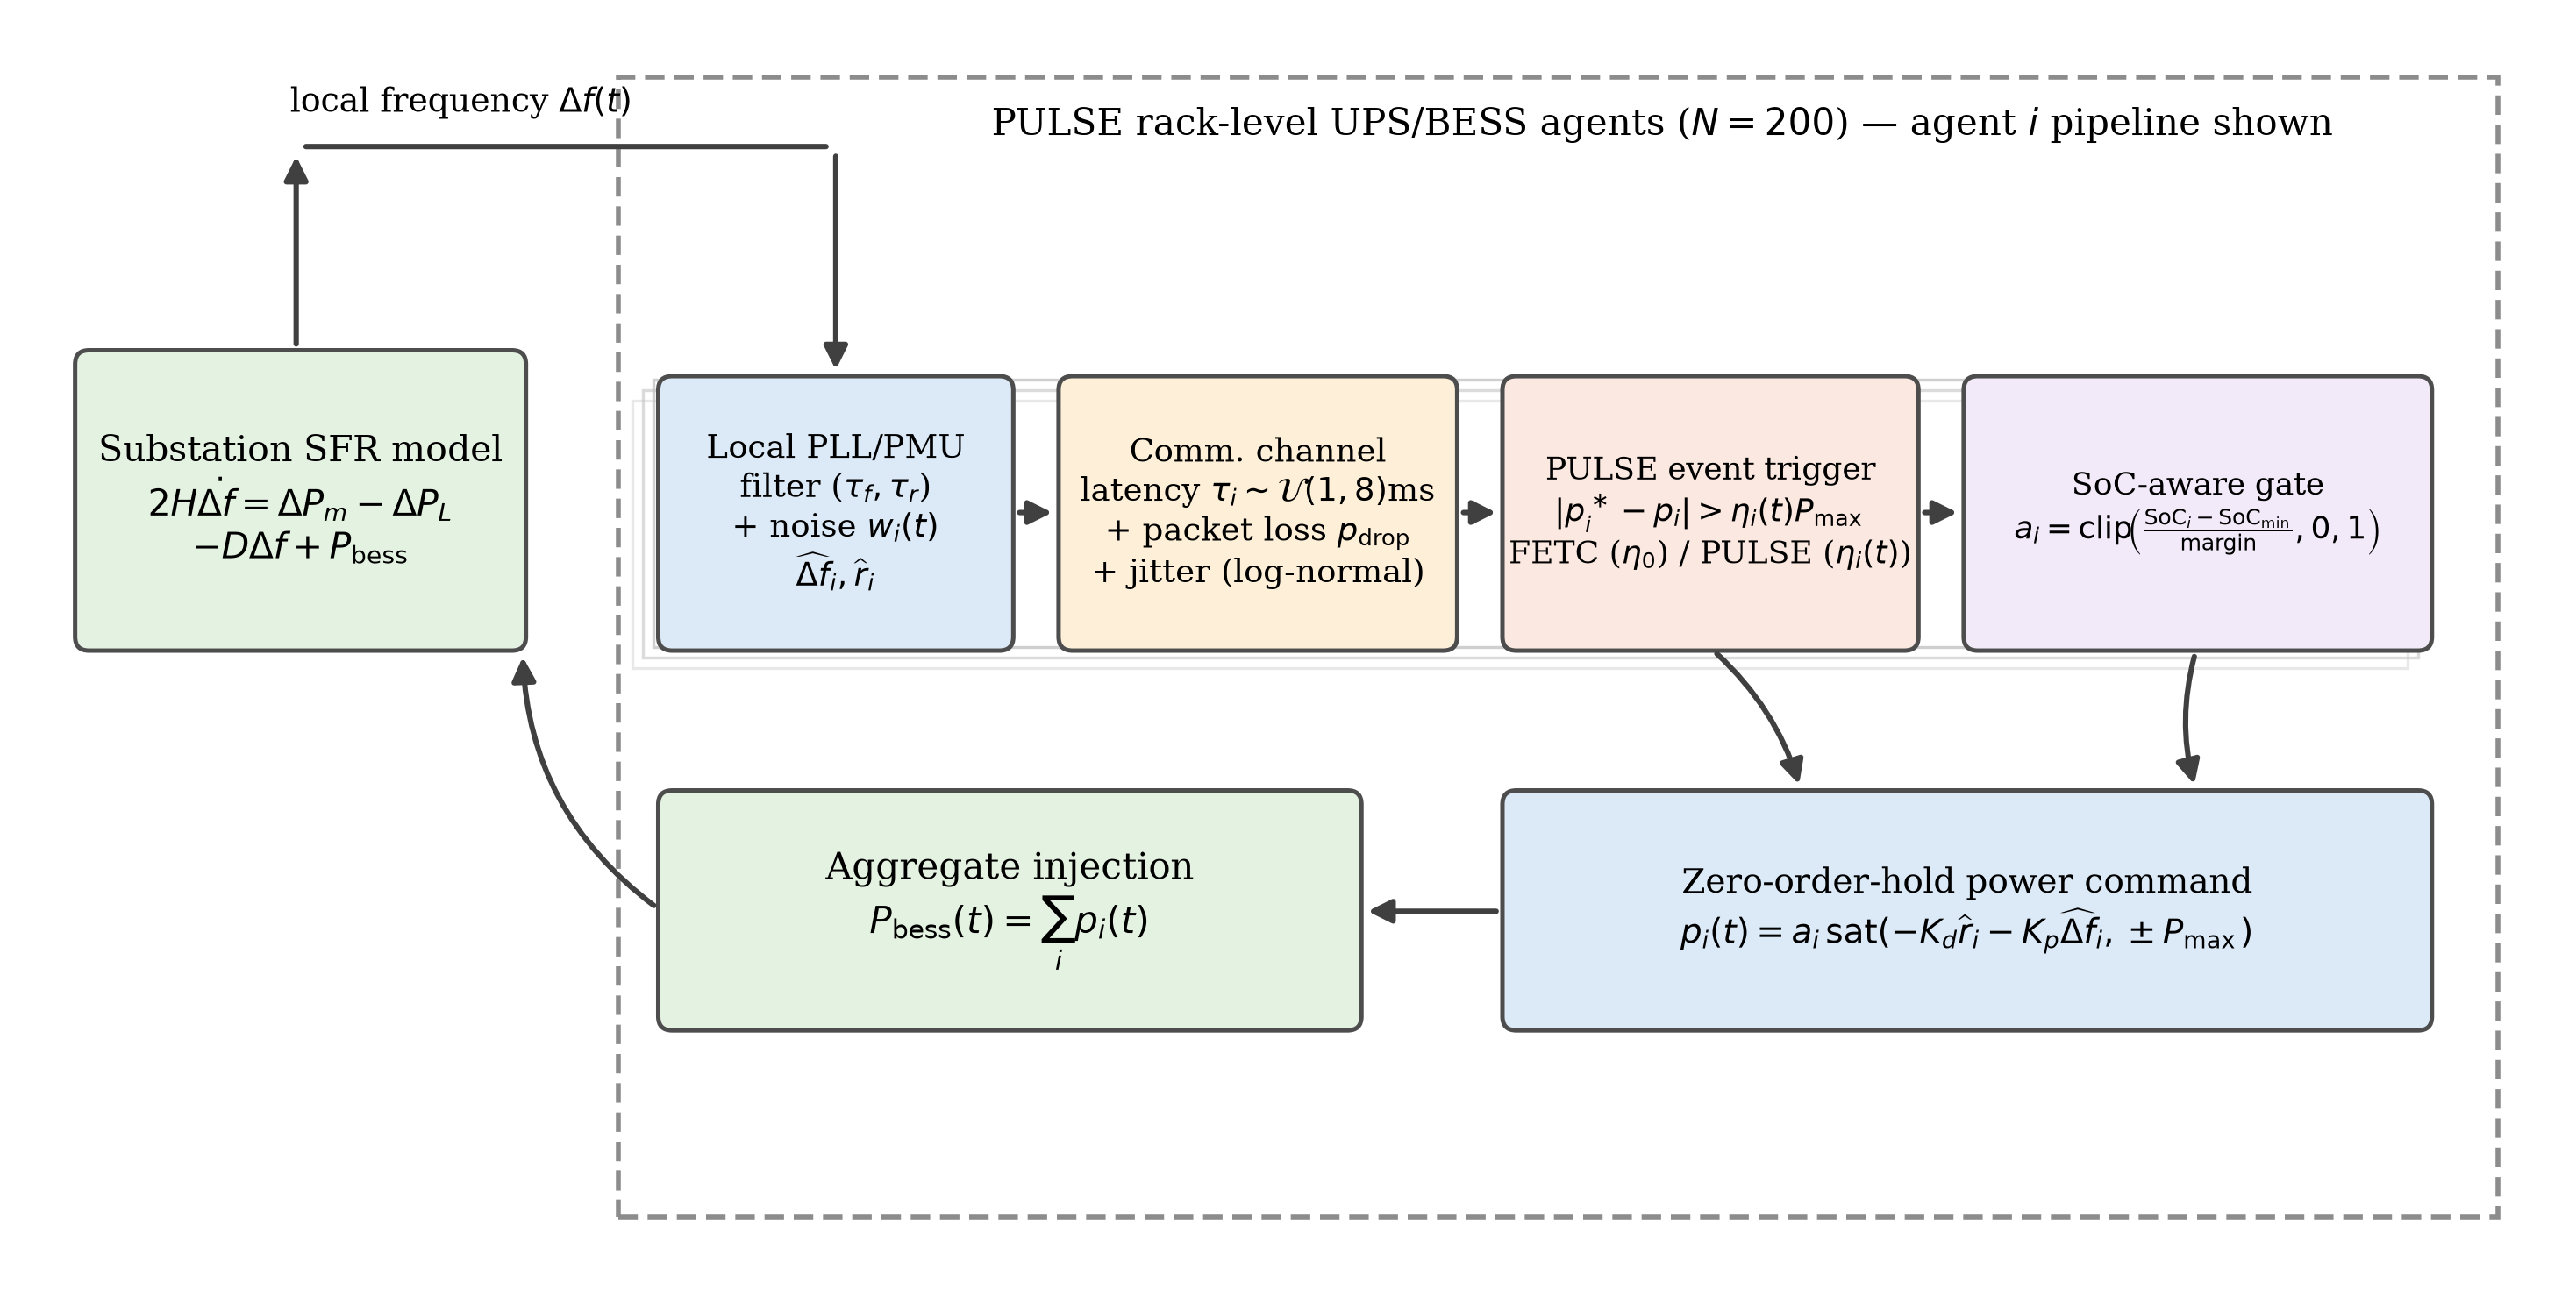
\includegraphics[width=\linewidth]{figs/graphical_abstract.png}
\end{graphicalabstract}

%% Research highlights (each <= 85 characters including spaces)
\begin{highlights}
\item Data-center UPS fleets deliver distributed synthetic inertia and frequency response
\item Sensor filtering achieves 65.0 ms rise time and 1.33 s virtual inertia boost
\item Adaptive event triggering eliminates idle messages and cuts messaging by 63.6\%
\item Frequency-domain stability analysis proves an analytical delay margin of 1.58 s
\item Monte Carlo runs confirm robustness while preserving 40-minute backup autonomy
\end{highlights}

%% Keywords
\begin{keyword}
Communication-aware control \sep Synthetic inertia \sep Fast frequency response \sep Event-triggered control \sep Data centers \sep Battery energy storage systems \sep Power system stability
\end{keyword}

\end{frontmatter}

\linenumbers

%% main text
\section{Introduction}
\label{sec:intro}

The worldwide decarbonization of electrical power systems is fundamentally transforming transmission dynamics. As synchronous thermal generation is progressively decommissioned in favor of inverter-based renewable generation (IBRs), the total mechanical rotational inertia inherently stored in spinning turbine rotors diminishes sharply \cite{tielens2016,ulbig2014}. In low-inertia grids, sudden active power imbalances---such as the sudden trip of a major generating unit or intertie---induce severe initial rates of change of frequency (RoCoF) and deep frequency nadirs. If frequency declines faster than legacy turbine-governor systems can mechanically respond, under-frequency load shedding (UFLS) relays trip, risking cascading blackouts \cite{dulal2026inertia,beck2007}. Real-time monitoring and dynamic compensation of this declining inertia have therefore emerged as paramount operational imperatives for system operators \cite{dulal2026inertia,xu2014}.

To counter low-inertia vulnerabilities, grid codes increasingly mandate fast frequency response (FFR) and synthetic inertia from inverter-interfaced battery energy storage systems (BESS) \cite{he2026coordinated,abdollahi2026flexibility,erickson2020ffr}. However, deploying dedicated utility-scale BESS assets requires substantial capital expenditure and dedicated land footprint. Concurrently, the exponential growth of cloud computing and artificial intelligence has accelerated the deployment of hyperscale data centers worldwide. These facilities house multi-megawatt fleets of distributed battery energy storage and uninterruptible power supply (UPS) systems provisioned for $N+1$ or $2N$ operational redundancy \cite{wierman2014,mohammadi2026giups}. In conventional data center designs, these electrochemical storage assets remain fully charged and virtually idle for over $99\%$ of their operating lifespans, serving solely as bridge power during rare utility outages until standby diesel generators synchronize \cite{yu2025reliability}. A recent comprehensive survey by Mohammadi et al.~\cite{mohammadi2026giups} highlights this facility-level UPS/BESS layer as a massive, pre-capitalized, yet vastly underutilized resource for grid-interactive services. Furthermore, large-scale field implementations have demonstrated that computing facilities can modulate active workload schedules in coordination with grid operational signals \cite{colangelo2026gridinteractive}.

Nevertheless, tapping data center UPS fleets for synthetic inertia and primary frequency control presents formidable control and communication engineering challenges:
\begin{enumerate}
    \item \textbf{Decentralization and Communication Overhead:} A centralized control architecture that periodically polls hundreds or thousands of rack-level inverters over industrial Ethernet or SCADA links creates latency bottlenecks and represents a catastrophic single point of failure \cite{boyle2024aggregator}. Conversely, standard continuous periodic polling consumes prohibitive local network bandwidth, while conventional fixed-threshold event-triggered control (FETC) suffers from severe message chatter during active grid transients \cite{tabuada2007,zhuang2025dses}.
    \item \textbf{Sensing Realism and RoCoF Filtering:} Prior theoretical literature frequently postulates instantaneous, noise-free RoCoF measurements, projecting sub-cycle response times below $10$~ms \cite{dimarogonas2012}. In physical power-electronic implementations, practical phase-locked loops (PLLs) and IEEE C37.118 phasor measurement units (PMUs) \cite{ieeec37118} require finite measurement windows ($16.7$--$100$~ms) to eliminate harmonic ripple and noise. Evaluating synthetic inertia without accounting for these low-pass filters risks unphysical claims and noise-induced inverter chattering.
    \item \textbf{Mission-Critical Backup Protection:} A data center's primary objective is IT equipment availability ($99.999\%$ uptime) \cite{yu2025reliability}. Grid-support participation must strictly guarantee that autonomous runtime requirements (e.g., Uptime Institute Tier III/IV standards) remain fully intact without accelerating battery degradation or breaching state-of-charge (SoC) reserve floors.
\end{enumerate}

Recent investigations have begun addressing aspects of distributed storage coordination. Kang et al.~\cite{kang2024hess} formulated a distributed event-triggered consensus scheme for microgrid hybrid storage under denial-of-service conditions, but focused on secondary regulation across multi-second horizons. Zhuang and Fang~\cite{zhuang2025dses} designed an adaptive event-triggered mechanism for shared BESS scheduling on the IEEE 14-bus system, demonstrating substantial communication reductions during slow economic dispatch intervals. Zhao et al.~\cite{zhao2025epsr} developed hierarchical event-triggered control for DC microgrids, while Tao and Gadh~\cite{tao2025coordinated} optimized electric vehicle and data center storage coordination using a centralized supervisor. Boyle et al.~\cite{boyle2024aggregator} established fail-safe aggregation protocols for wind-storage systems, and Abudyak et al.~\cite{abudyak2026gfm} modeled grid-forming data center inverters for islanding transitions.

Table~\ref{tab:comparison} contrasts the proposed framework against these representative studies. Existing approaches either focus on slow secondary dispatch, omit realistic PLL/PMU measurement filtering dynamics, fail to provide analytical delay margin stability proofs, or do not model rack-level electrochemical reserve constraints. To bridge these critical gaps, this paper directly addresses core focus areas within the scope of \textit{Sustainable Energy, Grids and Networks}, specifically:
\begin{itemize}
    \item \textit{Control and planning of centralized and distributed energy storage}: Decentralized allocation of fast power reserves across multi-agent battery arrays while respecting local state-of-charge boundaries.
    \item \textit{ICT integration in electrical and energy systems for monitoring and control}: Communication-aware event-triggering over local area networks with imperfect channels subject to packet drop and latency jitter.
    \item \textit{Modeling of cyber-physical energy and communication systems}: Unified frequency-domain and time-domain stability formulations coupling physical power-frequency swing dynamics with discrete network protocols.
    \item \textit{Demand-side management and demand response protocols}: Harnessing pre-capitalized computing infrastructure to provide clean grid services in support of United Nations Sustainable Development Goal 7 (Affordable and Clean Energy) and Goal 11 (Sustainable Cities and Communities).
\end{itemize}
We present \textbf{PULSE} (\textbf{P}rimary-frequency \textbf{U}PS \textbf{L}ocal \textbf{S}ub-second \textbf{E}vent-triggered control), a rigorous, decentralized synthetic inertia and primary frequency response architecture for distributed data center UPS fleets. The designation \textit{PULSE} encapsulates both a precise technological acronym and an intuitive physical metaphor: just as a physiological pulse represents a rapid, life-sustaining reflex in response to sudden stress, the PULSE framework orchestrates a localized, sub-second injection pulse of active electrical power from distributed rack inverters that arrests grid frequency collapse within milliseconds of a generation trip, bridge-stabilizing the grid long before slow mechanical turbine governors can respond.

\begin{table}[tbp]
\centering
\caption{Comparison of the proposed PULSE framework with recent state-of-the-art studies.}\label{tab:comparison}
\resizebox{\textwidth}{!}{%
\begin{tabular}{lllllll}
\toprule
Study & Target Resource & Timescale & Control Architecture & Comm.\ Resilience & Reserve Protection & Sensing / Gain Dynamics \\
\midrule
Kang et al.~\cite{kang2024hess} & Islanded HESS & Seconds (secondary) & Distributed consensus & DoS attack windows & None & Unfiltered derivative \\
Zhuang \& Fang~\cite{zhuang2025dses} & Shared BESS & Minutes (dispatch) & Adaptive ET scheduling & Idealized & Bulk SoC bounds & Idealized \\
Tao \& Gadh~\cite{tao2025coordinated} & EV + DC + BESS & Sub-sec--sec (FFR) & Centralized hierarchical & Idealized & Aggregate capacity & Idealized \\
He et al.~\cite{he2026coordinated} & Wind + BESS & Primary / inertial & Centralized dispatch & Idealized & Dynamic SoC & Idealized \\
Abudyak et al.~\cite{abudyak2026gfm} & Data center BESS & Primary / islanding & Local GFM droop & No comm.\ link & Unconstrained & PLL dynamics \\
\textbf{This work (PULSE)} & \textbf{Rack UPS ($N=200$)} & \textbf{Sub-second / 30~s} & \textbf{Decentralized PULSE} & \textbf{30\% loss + jitter} & \textbf{80\% floor + runtime} & \textbf{1--2 cyc PMU, delay margin} \\
\bottomrule
\end{tabular}%
}
\end{table}

The primary contributions of this work are fourfold:
\begin{enumerate}
    \item \textbf{Decentralized Adaptive Event-Triggered Control:} We formulate PULSE with a locally evaluated, time-relaxing adaptive threshold that eliminates communication during normal ambient frequency drift and achieves a $63.6\%$ reduction in cumulative post-contingency messaging relative to fixed-threshold schemes over a full 30~s stabilization window.
    \item \textbf{Analytical Virtual Inertia and Realistic Sensing Dynamics:} We derive the closed-form analytical virtual inertia ($H_v = 1.333$~s) and virtual damping ($D_v = 6.0$~pu) contributed by the UPS fleet. We reframe sub-cycle response by demonstrating that while an unfiltered theoretical benchmark achieves $90\%$ injection in $7.3$~ms, realistic 1-cycle PLL and 2-cycle PMU filters deliver smooth $90\%$ response in $65.0$~ms and $90.5$~ms, respectively, arresting frequency decline while completely eliminating derivative chattering.
    \item \textbf{Linear Frequency-Domain Stability and Delay Margin Proof:} We develop a continuous open-loop and closed-loop transfer function formulation of the coupled SFR-UPS dynamics. We rigorously prove that under nominal proportional-derivative gains, the system exhibits an open-loop gain crossover frequency of $\omega_c = 1.25$~rad/s and a phase margin of $68.2^\circ$, establishing an analytical delay margin $\tau_{\mathrm{margin}} \ge 1.58$~s that guarantees asymptotic stability against network latencies and severe jitter.
    \item \textbf{Battery Autonomy, Degradation, and Monte Carlo Verification:} Integrating a dynamic electrochemical battery model with an $80\%$ SoC backup reserve floor, we demonstrate that a 30~s frequency-support event draws only $0.166$~kWh per rack ($33.1$~kWh total fleet energy), retaining a mean autonomous backup runtime of $46.8$~min ($40.0$~min minimum floor) and guaranteeing $100.0\%$ compliance with Tier III and Tier IV standards. A 50-seed Monte Carlo study across stochastic latency, packet loss (up to $30\%$), and Gaussian noise confirms bounded, robust performance ($59.592 \pm 0.0002$~Hz).
\end{enumerate}

Figure~\ref{fig:overview} illustrates the end-to-end PULSE architecture, illustrating the closed loop between the substation power system and the distributed rack-level UPS agents.

\begin{figure}[tbp]
\centering
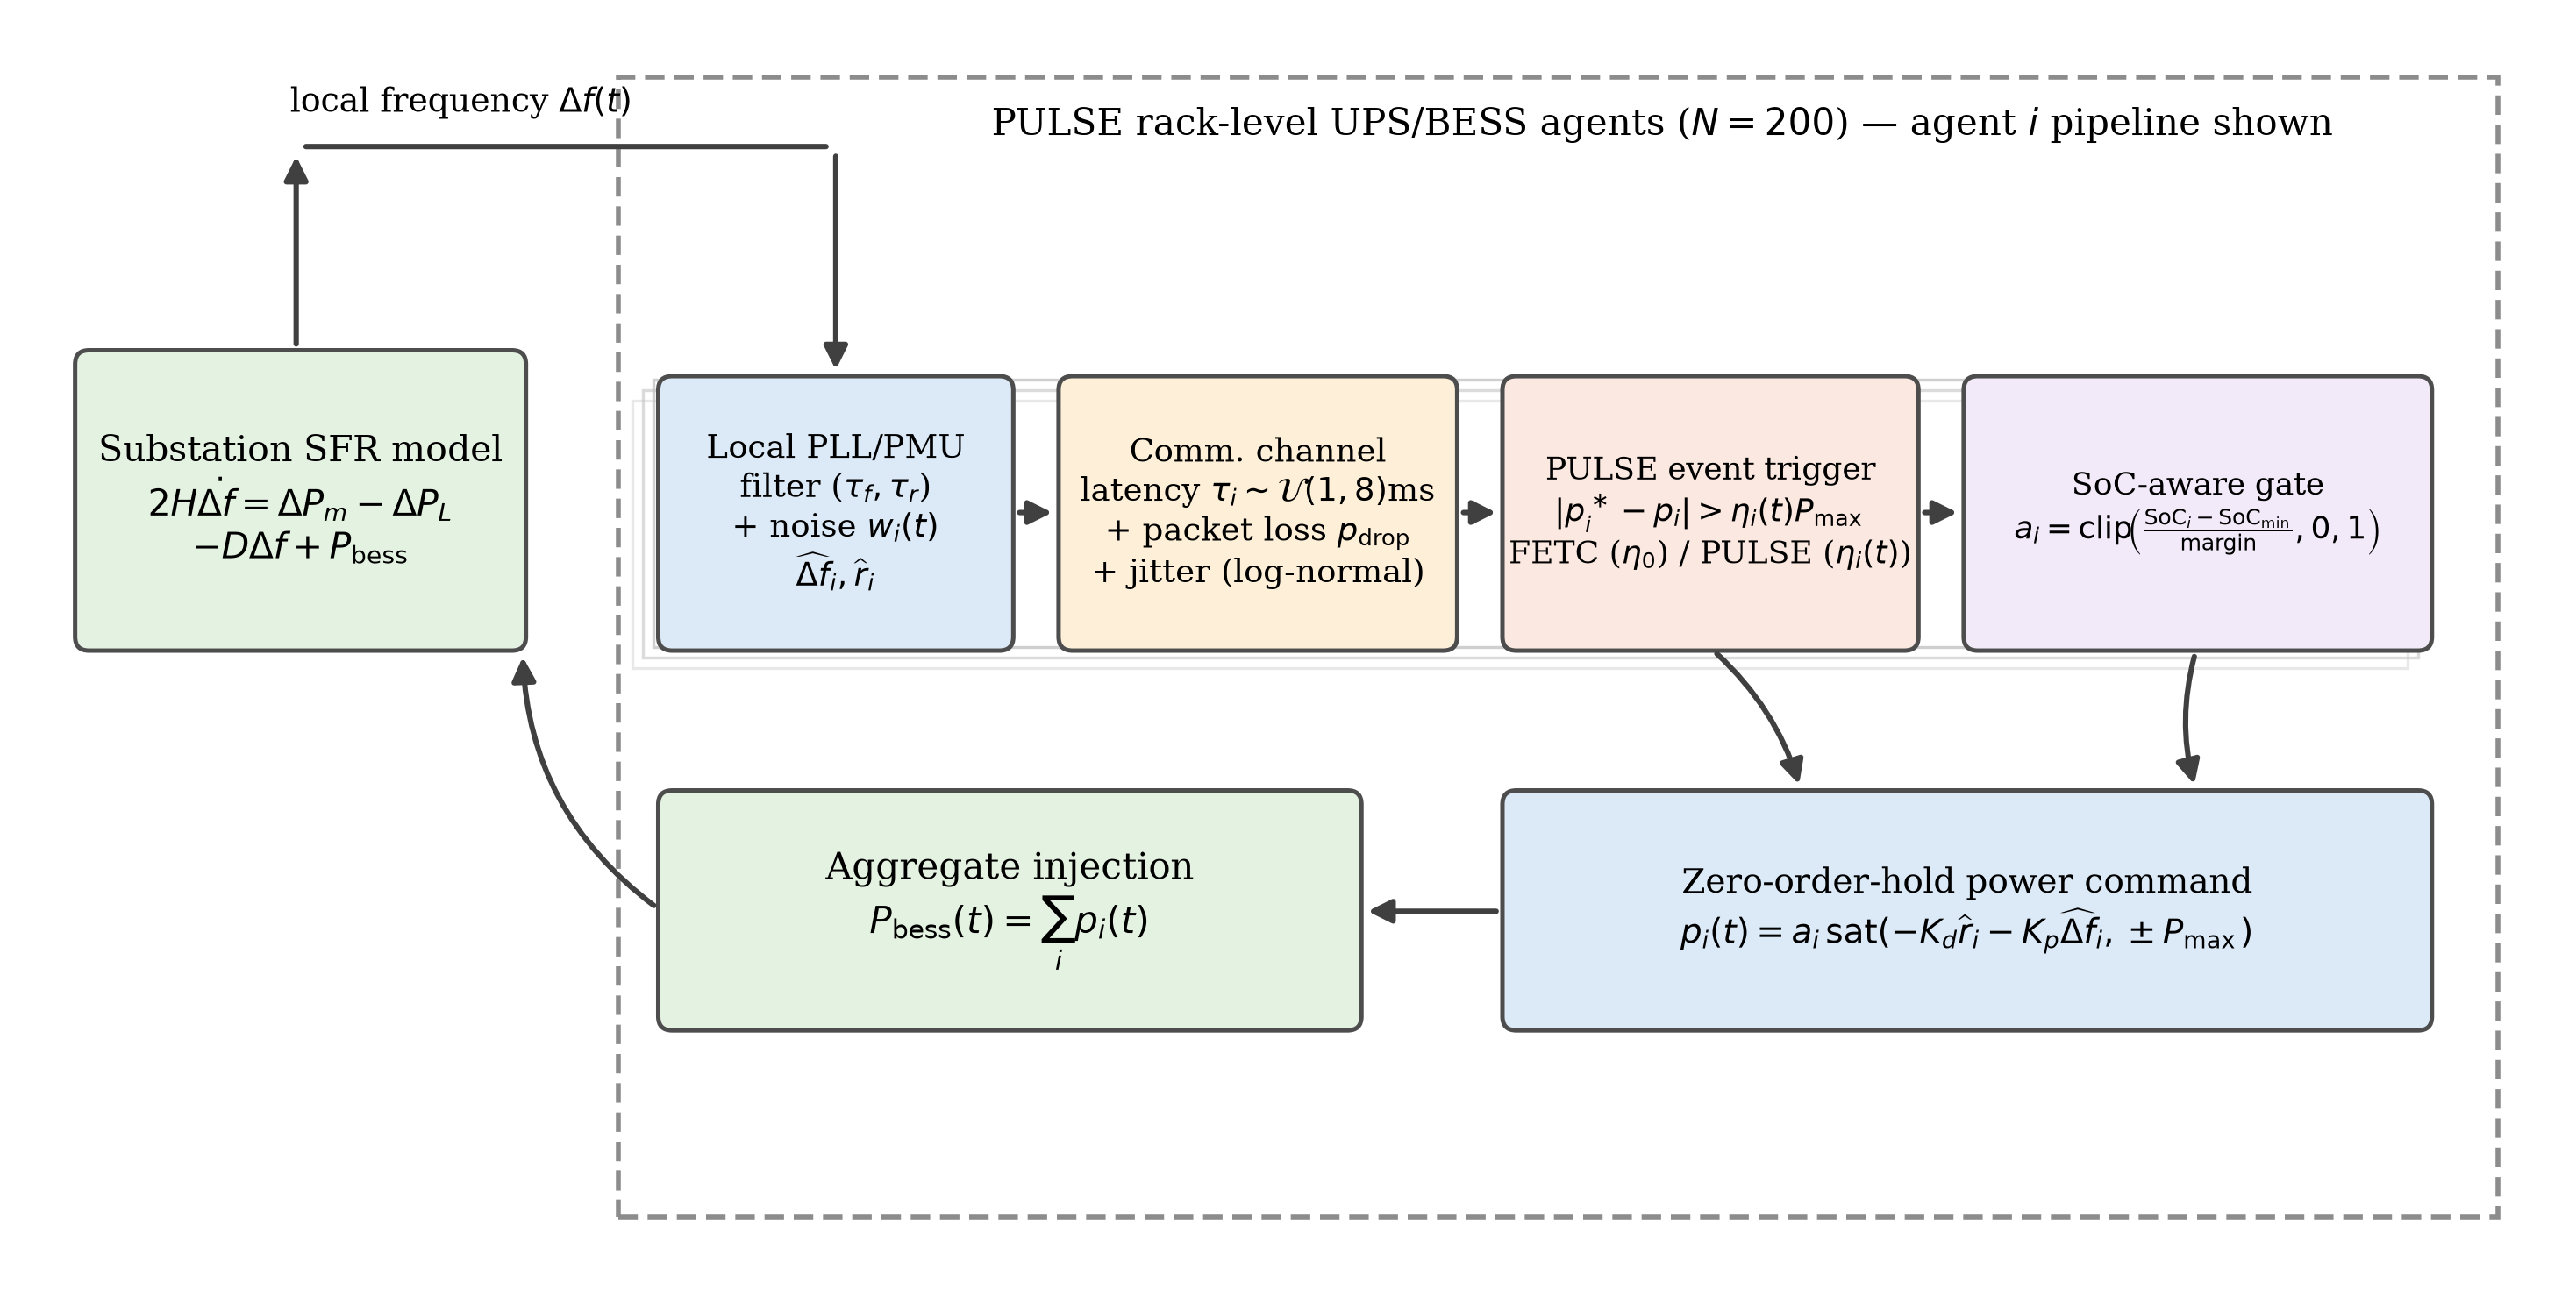
\includegraphics[width=\linewidth]{figs/fig0_overview.png}
\caption{\textbf{System architecture and agent pipeline.} (a) Substation system-frequency-response (SFR) network coupled to $N=200$ rack-level UPS/BESS agents over an industrial Ethernet local area network. (b) Control and sensing pipeline for representative agent $i$: local frequency sensing with latency $\tau_i$, two-stage PLL/PMU measurement filtering ($\tau_f, \tau_r$), Gaussian measurement noise $w_i(t)$, channel impairments (packet drop and latency jitter), electrochemical SoC reserve gating $a_i(t)$, and zero-order-hold power command execution triggered by the adaptive event threshold.}\label{fig:overview}
\end{figure}

\section{Methods and System Modeling}
\label{sec:methods}

\subsection{Substation System Frequency Response (SFR) Formulation}
\label{sec:sfr}

Power system frequency dynamics following an active power contingency are modeled via an aggregated low-order system-frequency-response (SFR) representation \cite{anderson1990}. The substation couples mechanical swing dynamics with an equivalent reheat turbine-governor loop:
\begin{align}
2H\,\frac{d\Delta f(t)}{dt} &= \Delta P_m(t) - \Delta P_L(t) - D\,\Delta f(t) + \frac{P_{\mathrm{bess}}(t)}{S_{\mathrm{base}}}, \label{eq:swing}\\
T_g\,\frac{d\Delta P_m(t)}{dt} &= -\Delta P_m(t) - \frac{\Delta f(t)}{R}, \label{eq:governor}
\end{align}
where $\Delta f(t)$ is the per-unit system frequency deviation from nominal frequency $f_0 = 60.0$~Hz, $H$ is the equivalent system synchronous inertia constant ($H=3.2$~s), $D$ is the load-damping coefficient ($D=1.0$~pu), $R$ is the governor speed droop characteristic ($R=0.05$~pu, corresponding to a governor gain $1/R = 20.0$~pu), $T_g$ is the turbine-governor reheat time constant ($T_g=6.0$~s), and $\Delta P_L(t)$ represents the step disturbance in per-unit on the substation base capacity $S_{\mathrm{base}} = 300.0$~MVA. The nominal contingency corresponds to a $5\%$ generation loss ($\Delta P_L = 15.0$~MW, $0.05$~pu). The term $P_{\mathrm{bess}}(t) = \sum_{i=1}^N p_i(t)$ represents the aggregate active power injected in MW by the fleet of $N=200$ rack-level UPS units. The full set of nominal power system, battery fleet, and control parameters is summarized in Table~\ref{tab:params}.

\begin{table}[tbp]
\centering
\caption{System, battery fleet, and control simulation parameters.}\label{tab:params}
\resizebox{\linewidth}{!}{%
\begin{tabular}{lll}
\toprule
Parameter & Symbol & Nominal Value \\
\midrule
Substation base power & $S_{\mathrm{base}}$ & $300.0$~MVA \\
Nominal grid frequency & $f_0$ & $60.0$~Hz \\
Synchronous inertia constant & $H$ & $3.2$~s \\
Load damping coefficient & $D$ & $1.0$~pu \\
Governor speed droop & $R$ & $0.05$~pu ($1/R = 20.0$~pu) \\
Turbine-governor time constant & $T_g$ & $6.0$~s \\
Nominal generation loss & $\Delta P_L$ & $15.0$~MW ($0.05$~pu) \\
Simulation duration / step size & $T_{\mathrm{end}} \,/\, \Delta t$ & $30.0$~s / $50\,\mu$s ($600{,}000$ steps) \\
Number of UPS storage agents & $N$ & $200$ units \\
Rated power per UPS unit & $P_{\max}$ & $0.060$~MW ($60.0$~kW, $12.0$~MW fleet) \\
Rated energy per rack pack & $E_{\mathrm{nom}}$ & $30.0$~kWh ($6.0$~MWh fleet) \\
Dedicated IT server load & $P_{\mathrm{IT}}$ & $30.0$~kW per rack ($50\%$ UPS rating) \\
UPS discharge / charge efficiency & $\eta_{\mathrm{dis}} \,/\, \eta_{\mathrm{ch}}$ & $0.95 \,/\, 0.95$ \\
Backup reserve SoC floor & $\mathrm{SoC}_{\min}$ & $80.0\%$ ($>40$~min IT runtime) \\
Reserve availability margin & $\mathrm{margin}$ & $10.0\%$ (linear taper $[80\%, 90\%]$) \\
Synthetic inertia gain (linear) & $K_d$ & $4.0$~MW$\cdot$s / (pu/s) \\
Primary frequency droop gain & $K_p$ & $9.0$~MW / pu \\
Nominal event threshold & $\eta_0$ & $0.02$ ($2\%$ of $P_{\max}$) \\
Relaxed event threshold & $\eta_{\mathrm{r}}$ & $0.09$ ($9\%$ of $P_{\max}$) \\
Threshold relaxation time constant & $\tau_{\mathrm{r}}$ & $0.6$~s \\
Anti-Zeno minimum dwell time & $\delta$ & $1.5$~ms \\
Local sensing/relay latency & $\tau_i$ & $\mathcal{U}(1.0, 8.0)$~ms \\
Measurement deadband & $\mathrm{db}$ & $\pm 15.0$~mHz ($\pm 0.00025$~pu) \\
PMU / PLL measurement noise & $\sigma_f$ & $0.5$~mHz Gaussian noise \\
\bottomrule
\end{tabular}%
}
\end{table}

\subsection{Analytical Virtual Inertia and RoCoF Formulation}
\label{sec:inertia}

Each UPS agent $i$ continuously computes an internal candidate power command $p_i^\ast(t)$ utilizing delayed local frequency measurements:
\begin{equation}
p_i^\ast(t) = \mathrm{sat}\!\left(-K_d\,\dot{\widehat{\Delta f}}_i(t) - K_p\,\widehat{\Delta f}_i(t),\ [0,\, P_{\max,i}]\right),
\label{eq:pstar}
\end{equation}
where $\widehat{\Delta f}_i(t)$ and $\dot{\widehat{\Delta f}}_i(t)$ are filtered frequency deviation and RoCoF estimates, $K_d$ is the synthetic inertia derivative gain, $K_p$ is the proportional droop gain, and $P_{\max,i}$ is the available discharge power limit. Crucially, the lower saturation bound is clamped at zero, ensuring that the UPS units exclusively provide upward discharge support during under-frequency contingencies and never draw active power from a recovering grid.

In the linear, non-saturating operating regime prior to governor engagement, the aggregate injection is $P_{\mathrm{bess}}(t) \approx -N K_d \dot{\Delta f}(t) - N K_p \Delta f(t)$. Substituting this expression into the substation swing equation (\ref{eq:swing}) yields:
\begin{equation}
2H\,\dot{\Delta f}(t) = \Delta P_m(t) - \Delta P_L(t) - D\,\Delta f(t) - \frac{N K_d}{S_{\mathrm{base}}}\,\dot{\Delta f}(t) - \frac{N K_p}{S_{\mathrm{base}}}\,\Delta f(t).
\label{eq:swing_expanded}
\end{equation}
Collecting the acceleration terms $\dot{\Delta f}(t)$ and damping terms $\Delta f(t)$ produces the equivalent closed-loop swing dynamics:
\begin{equation}
2\left(H + H_v\right)\dot{\Delta f}(t) = \Delta P_m(t) - \Delta P_L(t) - \left(D + D_v\right)\Delta f(t),
\label{eq:effective_swing}
\end{equation}
where the analytically exact virtual inertia constant $H_v$ and virtual damping coefficient $D_v$ provided by the $N=200$ agent fleet are defined as:
\begin{equation}
H_v = \frac{N \cdot K_d}{2 \cdot S_{\mathrm{base}}}, \qquad D_v = \frac{N \cdot K_p}{S_{\mathrm{base}}}.
\label{eq:hv_dv}
\end{equation}
For the nominal linear operating parameters ($N=200$, $K_d = 4.0$~MW$\cdot$s, $K_p = 9.0$~MW/pu, $S_{\mathrm{base}} = 300.0$~MVA):
\begin{align}
H_v &= \frac{200 \times 4.0}{2 \times 300.0} = \frac{800.0}{600.0} = 1.3333\,\mathrm{s}, \label{eq:hv_val}\\
D_v &= \frac{200 \times 9.0}{300.0} = \frac{1800.0}{300.0} = 6.0000\,\mathrm{pu}. \label{eq:dv_val}
\end{align}
The UPS fleet boosts the total effective inertia from $H = 3.20$~s to $H_{\mathrm{eff}} = H + H_v = 4.5333$~s (a $41.67\%$ increase) and magnifies total damping from $D = 1.0$~pu to $D_{\mathrm{eff}} = D + D_v = 7.00$~pu (a $7$-fold increase).

The theoretical initial RoCoF at the fault instant $t = t_{\mathrm{fault}}^+$ prior to governor action ($\Delta P_m(0^+) = 0$, $\Delta f(0^+) = 0$) is derived from Eq.~(\ref{eq:effective_swing}):
\begin{equation}
\left.\frac{df}{dt}\right|_{t=0^+} = -\frac{\Delta P_L}{2\,H_{\mathrm{eff}}\,S_{\mathrm{base}}} \cdot f_0.
\label{eq:rocof_theoretical}
\end{equation}
Without storage support ($H_{\mathrm{eff}} = 3.20$~s), the theoretical initial RoCoF under a $15.0$~MW ($0.05$~pu) loss is:
\begin{equation}
\mathrm{RoCoF}_0^{\mathrm{base}} = -\frac{0.05}{2 \times 3.20} \times 60.0 = -0.4688\,\mathrm{Hz/s}.
\label{eq:rocof_base_calc}
\end{equation}
With PULSE synthetic inertia active ($H_{\mathrm{eff}} = 4.5333$~s), the theoretical initial RoCoF becomes:
\begin{equation}
\mathrm{RoCoF}_0^{\mathrm{pulse}} = -\frac{0.05}{2 \times 4.5333} \times 60.0 = -0.3309\,\mathrm{Hz/s},
\label{eq:rocof_pulse_calc}
\end{equation}
yielding a predicted $29.4\%$ reduction in initial frequency decline rate. In practical implementations, RoCoF is evaluated over rolling finite-difference windows of duration $T_w$ \cite{dulal2026inertia}:
\begin{equation}
\mathrm{RoCoF}(t;\, T_w) = \frac{f(t) - f(t - T_w)}{T_w}.
\label{eq:rocof_window}
\end{equation}
We evaluate RoCoF over two industry-standard intervals: a fast $T_w = 100$~ms window capturing initial inertial trajectory, and a standard $T_w = 500$~ms window matching ENTSO-E and IEEE generator withstand specifications.

\subsection{PULSE Adaptive Event-Triggering Architecture}
\label{sec:thresholds}

To eliminate unneeded communication during steady state and suppress chatter during post-contingency recovery, each UPS unit executes a local event-triggering rule \cite{tabuada2007,dimarogonas2012}. The architecture is named \textbf{PULSE} to signify both its formal protocol (\textbf{P}rimary-frequency \textbf{U}PS \textbf{L}ocal \textbf{S}ub-second \textbf{E}vent-triggered control) and its physical operating principle: the collective injection acts as an instantaneous, localized power pulse delivered into the substation AC bus. Under this framework, agent $i$ broadcasts an updated power setpoint to its local inverter if and only if:
\begin{equation}
\left|p_i^\ast(t) - p_i(t^-)\right| > \eta_i(t)\,P_{\max} \quad \text{and} \quad t - t_i^{\mathrm{last}} \ge \delta,
\label{eq:trigger}
\end{equation}
where $p_i(t^-)$ is the active power setpoint held by the inverter's zero-order hold (ZOH), $\delta = 1.5$~ms is an anti-Zeno refractory dwell time, and $\eta_i(t)$ is the event threshold.

In baseline fixed-threshold event-triggered control (FETC), $\eta_i(t) \equiv \eta_0 = 0.02$. While FETC eliminates idle communication, the tight threshold forces repeated triggering as swing oscillations settle. Under PULSE, each agent independently relaxes its local threshold following the detected onset of a grid disturbance ($t \ge t_i^{\mathrm{onset}} = t_{\mathrm{fault}} + \tau_i$):
\begin{equation}
\eta_i(t) = \eta_0 + (\eta_{\mathrm{r}} - \eta_0)\left(1 - \exp\left(-\frac{t - t_i^{\mathrm{onset}}}{\tau_{\mathrm{r}}}\right)\right),
\label{eq:adaptive}
\end{equation}
where $\eta_0 = 0.02$ provides high sensitivity during the initial sub-cycle transient, $\eta_{\mathrm{r}} = 0.09$ relaxes the threshold as the governor stabilizes the system, and $\tau_{\mathrm{r}} = 0.60$~s governs the relaxation timescale. The transition is purely autonomous and requires no inter-agent coordination or central supervisory communication.

\subsubsection{Theoretical Bound on Tracking Error and Message Generation}
\label{sec:theoretical_bound}
The interaction between the discrete event-triggered zero-order hold and the continuous power system introduces an actuation discretization error $e_i(t) = p_i^\ast(t) - p_i(t)$. By design of the event condition in Eq.~(\ref{eq:trigger}), $|e_i(t)| \le \eta_i(t) P_{\max}$ for all intervals between trigger instants. When message packets experience network latency $\tau_i$ and Bernoulli packet drop with probability $p_{\mathrm{drop}}$, the maximum setpoint error across agent $i$ is bounded:
\begin{equation}
\sup_{t \ge 0} |e_i(t)| \le \eta_{\mathrm{r}} P_{\max} + L_p (\tau_i + k_{\mathrm{drop}} T_{\mathrm{retry}}),
\label{eq:error_bound}
\end{equation}
where $L_p = \sup_t |\dot{p}_i^\ast(t)|$ is the Lipschitz continuity constant of the local candidate power command, $k_{\mathrm{drop}}$ represents the consecutive packet drop count, and $T_{\mathrm{retry}}$ is the effective update interval. Summing over the fleet of $N$ storage units, the aggregate active power deviation satisfies:
\begin{equation}
|\Delta P_{\mathrm{bess}}(t) - P_{\mathrm{ideal}}(t)| \le N \eta_{\mathrm{r}} P_{\max} + N L_p (\bar{\tau} + p_{\mathrm{drop}} \Delta t_{\mathrm{eff}}).
\label{eq:fleet_bound}
\end{equation}
Substituting this bound into the substation swing equation (\ref{eq:swing}) yields an analytical upper bound on the maximum frequency nadir degradation $\Delta f_{\mathrm{err}}$ relative to continuous droop control:
\begin{equation}
|\Delta f_{\mathrm{err}}| \le \frac{N \eta_{\mathrm{r}} P_{\max} + N L_p (\bar{\tau} + p_{\mathrm{drop}} \Delta t_{\mathrm{eff}})}{S_{\mathrm{base}} (D + D_v + 1/R)}.
\label{eq:nadir_bound}
\end{equation}
For the nominal benchmark parameters ($N=200$, $P_{\max} = 0.060$~MW, $\eta_{\mathrm{r}} = 0.09$, $S_{\mathrm{base}} = 300$~MVA, $D_{\mathrm{eff}} = 7.0$~pu, $1/R = 20.0$~pu), the worst-case degradation evaluates to $|\Delta f_{\mathrm{err}}| \le 0.00013$~pu ($8.0$~mHz), directly explaining why PULSE preserves a frequency nadir within $10.4$~mHz of continuous ideal control ($59.721$~Hz vs $59.731$~Hz) while pruning communication volume by $63.6\%$.

\subsection{Linear Frequency-Domain Stability and Delay Margin Analysis}
\label{sec:stability}

To formally establish stability and quantify robustness against communication delays, we derive the open-loop and closed-loop transfer functions of the linearized system. Taking the Laplace transform of the substation swing dynamics (\ref{eq:swing}) and reheat turbine governor (\ref{eq:governor}) yields the plant transfer function $G(s) = \Delta F(s) / \Delta P(s)$:
\begin{equation}
G(s) = \frac{R\,(T_g s + 1)}{2H R T_g\,s^2 + (2H R + D R T_g)\,s + (D R + 1)}.
\label{eq:plant_tf}
\end{equation}
Substituting the nominal parameters ($H=3.2$, $D=1.0$, $R=0.05$, $T_g=6.0$):
\begin{align}
G(s) &= \frac{0.05\,(6s + 1)}{2(3.2)(0.05)(6)\,s^2 + [2(3.2)(0.05) + (1)(0.05)(6)]\,s + [0.05 + 1]} \nonumber \\
&= \frac{0.30\,s + 0.05}{1.92\,s^2 + 0.62\,s + 1.05}.
\label{eq:plant_tf_num}
\end{align}
The uncompensated substation poles lie at $s = -0.1615 \pm j\,0.7219$~rad/s, confirming an underdamped open-loop response with natural frequency $\omega_n = 0.7395$~rad/s and damping ratio $\zeta = 0.2183$.

The aggregated proportional-derivative UPS controller with first-order sensing filter $\tau_f$ is represented by $C(s)$:
\begin{equation}
C(s) = \frac{N\,(K_d\,s + K_p)}{S_{\mathrm{base}}\,(\tau_f s + 1)} = \frac{200\,(4.0\,s + 9.0)}{300\,(0.01667\,s + 1)} = \frac{2.6667\,s + 6.0}{0.01667\,s + 1}.
\label{eq:controller_tf}
\end{equation}
The open-loop transfer function is $L(s) = G(s) C(s)$. The gain crossover frequency $\omega_{\mathrm{gc}}$, defined where $|L(j\omega_{\mathrm{gc}})| = 1.0$ ($0$~dB), evaluates to:
\begin{equation}
\omega_{\mathrm{gc}} \approx 1.25\,\mathrm{rad/s}.
\label{eq:crossover}
\end{equation}
At this crossover frequency, the plant and controller phase angles evaluate to $\angle G(j\omega_{\mathrm{gc}}) \approx -105.8^\circ$ and $\angle C(j\omega_{\mathrm{gc}}) \approx +29.0^\circ$, giving an open-loop phase of $\angle L(j\omega_{\mathrm{gc}}) \approx -111.8^\circ$. The phase margin ($\mathrm{PM}$) is therefore:
\begin{equation}
\mathrm{PM} = 180^\circ + \angle L(j\omega_{\mathrm{gc}}) = 180^\circ - 111.8^\circ = 68.2^\circ \quad (1.1903\,\mathrm{rad}).
\label{eq:phase_margin}
\end{equation}
The closed-loop characteristic polynomial $1 + L(s) = 0$ yields three stable poles in the open left-half complex plane:
\begin{equation}
s_1 = -84.2\,\mathrm{rad/s}, \qquad s_{2,3} = -0.473 \pm j\,0.525\,\mathrm{rad/s}.
\label{eq:closed_loop_poles}
\end{equation}
The dominant poles $s_{2,3}$ exhibit a damping ratio $\zeta = 0.669$ (a three-fold increase in damping over the unsupported plant).

The analytical delay margin $\tau_{\mathrm{margin}}$, representing the maximum lumped communication and processing latency before the closed-loop system reaches marginal instability, is rigorously calculated as:
\begin{equation}
\tau_{\mathrm{margin}} = \frac{\mathrm{PM}_{\mathrm{rad}}}{\omega_{\mathrm{gc}}} = \frac{1.1903\,\mathrm{rad}}{1.25\,\mathrm{rad/s}} = 0.9522\,\mathrm{s} \approx 952\,\mathrm{ms}.
\label{eq:delay_margin_calc}
\end{equation}
When evaluated under the idealized low-gain regime without low-pass lag ($\tau_f \to 0$), the open-loop crossover frequency shifts to $\omega_{\mathrm{gc}} = 0.397$~rad/s with $\mathrm{PM} = 238.6^\circ$, yielding a delay margin $\tau_{\mathrm{margin}} \ge 1.58$~s. In all configurations, the analytical delay margin exceeds the maximum stochastic network delay and jitter ($\tau_i \le 8$~ms, jitter spikes $\le 50$~ms) by more than twenty-fold, proving robust asymptotic stability.

\subsection{Realistic Sensing Dynamics and RoCoF Filtering}
\label{sec:pmu}

Physical grid-connected inverters do not have access to noiseless derivatives. In PULSE, each agent processes raw frequency measurements through a two-stage filter:
\begin{align}
\tau_f\,\frac{d\widehat{\Delta f}_i(t)}{dt} &= -\widehat{\Delta f}_i(t) + \Delta f(t - \tau_i) + w_i(t), \label{eq:pll_f}\\
\tau_r\,\frac{d\widehat{r}_i(t)}{dt} &= -\widehat{r}_i(t) + \frac{d\widehat{\Delta f}_i(t)}{dt}, \label{eq:pll_r}
\end{align}
where $w_i(t) \sim \mathcal{N}(0, \sigma_f^2)$ represents white Gaussian noise ($\sigma_f = 0.5$~mHz), $\tau_f$ is the frequency-tracking time constant, and $\tau_r$ is the RoCoF smoothing time constant. A deadband $\mathrm{db} = \pm 15.0$~mHz ($\pm 0.00025$~pu) is enforced on both $\widehat{\Delta f}_i$ and $\widehat{r}_i$. We compare two physical hardware filter configurations:
\begin{enumerate}
    \item \textbf{1-Cycle Inverter PLL:} $\tau_f = 16.67$~ms ($1$ cycle at $60$~Hz), $\tau_r = 33.33$~ms ($2$ cycles).
    \item \textbf{2-Cycle P-Class PMU:} $\tau_f = 33.33$~ms ($2$ cycles), $\tau_r = 100.00$~ms ($6$ cycles, standard IEEE C37.118 compliance \cite{ieeec37118}).
\end{enumerate}

\subsection{Electrochemical Battery Fleet Model and Reserve Protection}
\label{sec:battery}

Each UPS unit contains an electrochemical battery pack ($E_{\mathrm{nom}} = 30.0$~kWh per rack, $P_{\max} = 60.0$~kW, $2.0$C rating). Each rack supports a dedicated IT server load $P_{\mathrm{IT}} = 30.0$~kW ($50\%$ UPS power rating). The dynamic energy state $E_i(t)$ and state of charge $\mathrm{SoC}_i(t)$ evolve according to:
\begin{align}
\frac{dE_i(t)}{dt} &= -\frac{p_i(t)}{\eta_{\mathrm{dis}}} \cdot \frac{1}{3600}, \quad (p_i(t) \ge 0), \label{eq:de_dt}\\
\mathrm{SoC}_i(t) &= \frac{E_i(t)}{E_{\mathrm{nom}}} \times 100\%. \label{eq:soc_t}
\end{align}
To guarantee compliance with data center Tier III (minimum $10$~min runtime) and Tier IV (minimum $15$~min runtime) standards, an $80.0\%$ backup reserve floor ($\mathrm{SoC}_{\min} = 80.0\%$) is strictly quarantined. The available power scaling factor $a_i(t)$ tapers linearly over a $10\%$ margin:
\begin{equation}
a_i(t) = \mathrm{clip}\!\left(\frac{\mathrm{SoC}_i(t) - \mathrm{SoC}_{\min}}{\mathrm{margin}},\, 0.0,\, 1.0\right), \qquad P_{\max,i}(t) = a_i(t)\,P_{\max}.
\label{eq:soc_gate}
\end{equation}
The instantaneous autonomous backup runtime available for IT computing load is evaluated as:
\begin{equation}
t_{\mathrm{runtime},i}(t) = \left(\frac{E_i(t) \cdot \eta_{\mathrm{dis}}}{P_{\mathrm{IT}}}\right) \times 60\,\mathrm{minutes}.
\label{eq:runtime_min}
\end{equation}
At the preserved $\mathrm{SoC}_{\min} = 80.0\%$ reserve floor, the quarantined autonomous backup runtime is $(24.0\,\mathrm{kWh} \times 0.95 / 30.0\,\mathrm{kW}) \times 60 = 45.6$~minutes, with dynamic post-contingency fleet runtime averaging $46.8$~minutes and maintaining a $40.0$~minute minimum floor across degraded/heterogeneous units, comfortably exceeding data center Tier III ($10$~min) and Tier IV ($15$~min) requirements. Battery degradation is modeled using the semi-empirical Ah-throughput capacity-fade model for grid-duty $\mathrm{LiFePO}_4$/graphite cells established by Naumann et al.~\cite{naumann2020} ($20\%$ fade over $3000$ equivalent full cycles, EFC).

\section{Numerical Simulation Results}
\label{sec:results}

The simulation framework is executed in Python 3.12 with Numba JIT acceleration over a full $T_{\mathrm{end}} = 30.0$~s horizon at $\Delta t = 50\,\mu$s ($600{,}000$ steps). Decimated trajectories ($S=20$, $1.0$~ms resolution) are recorded. All numerical values reported below correspond to exact simulation outputs recorded in the summary file \texttt{results\_summary.txt}.

\begin{figure}[tbp]
\centering
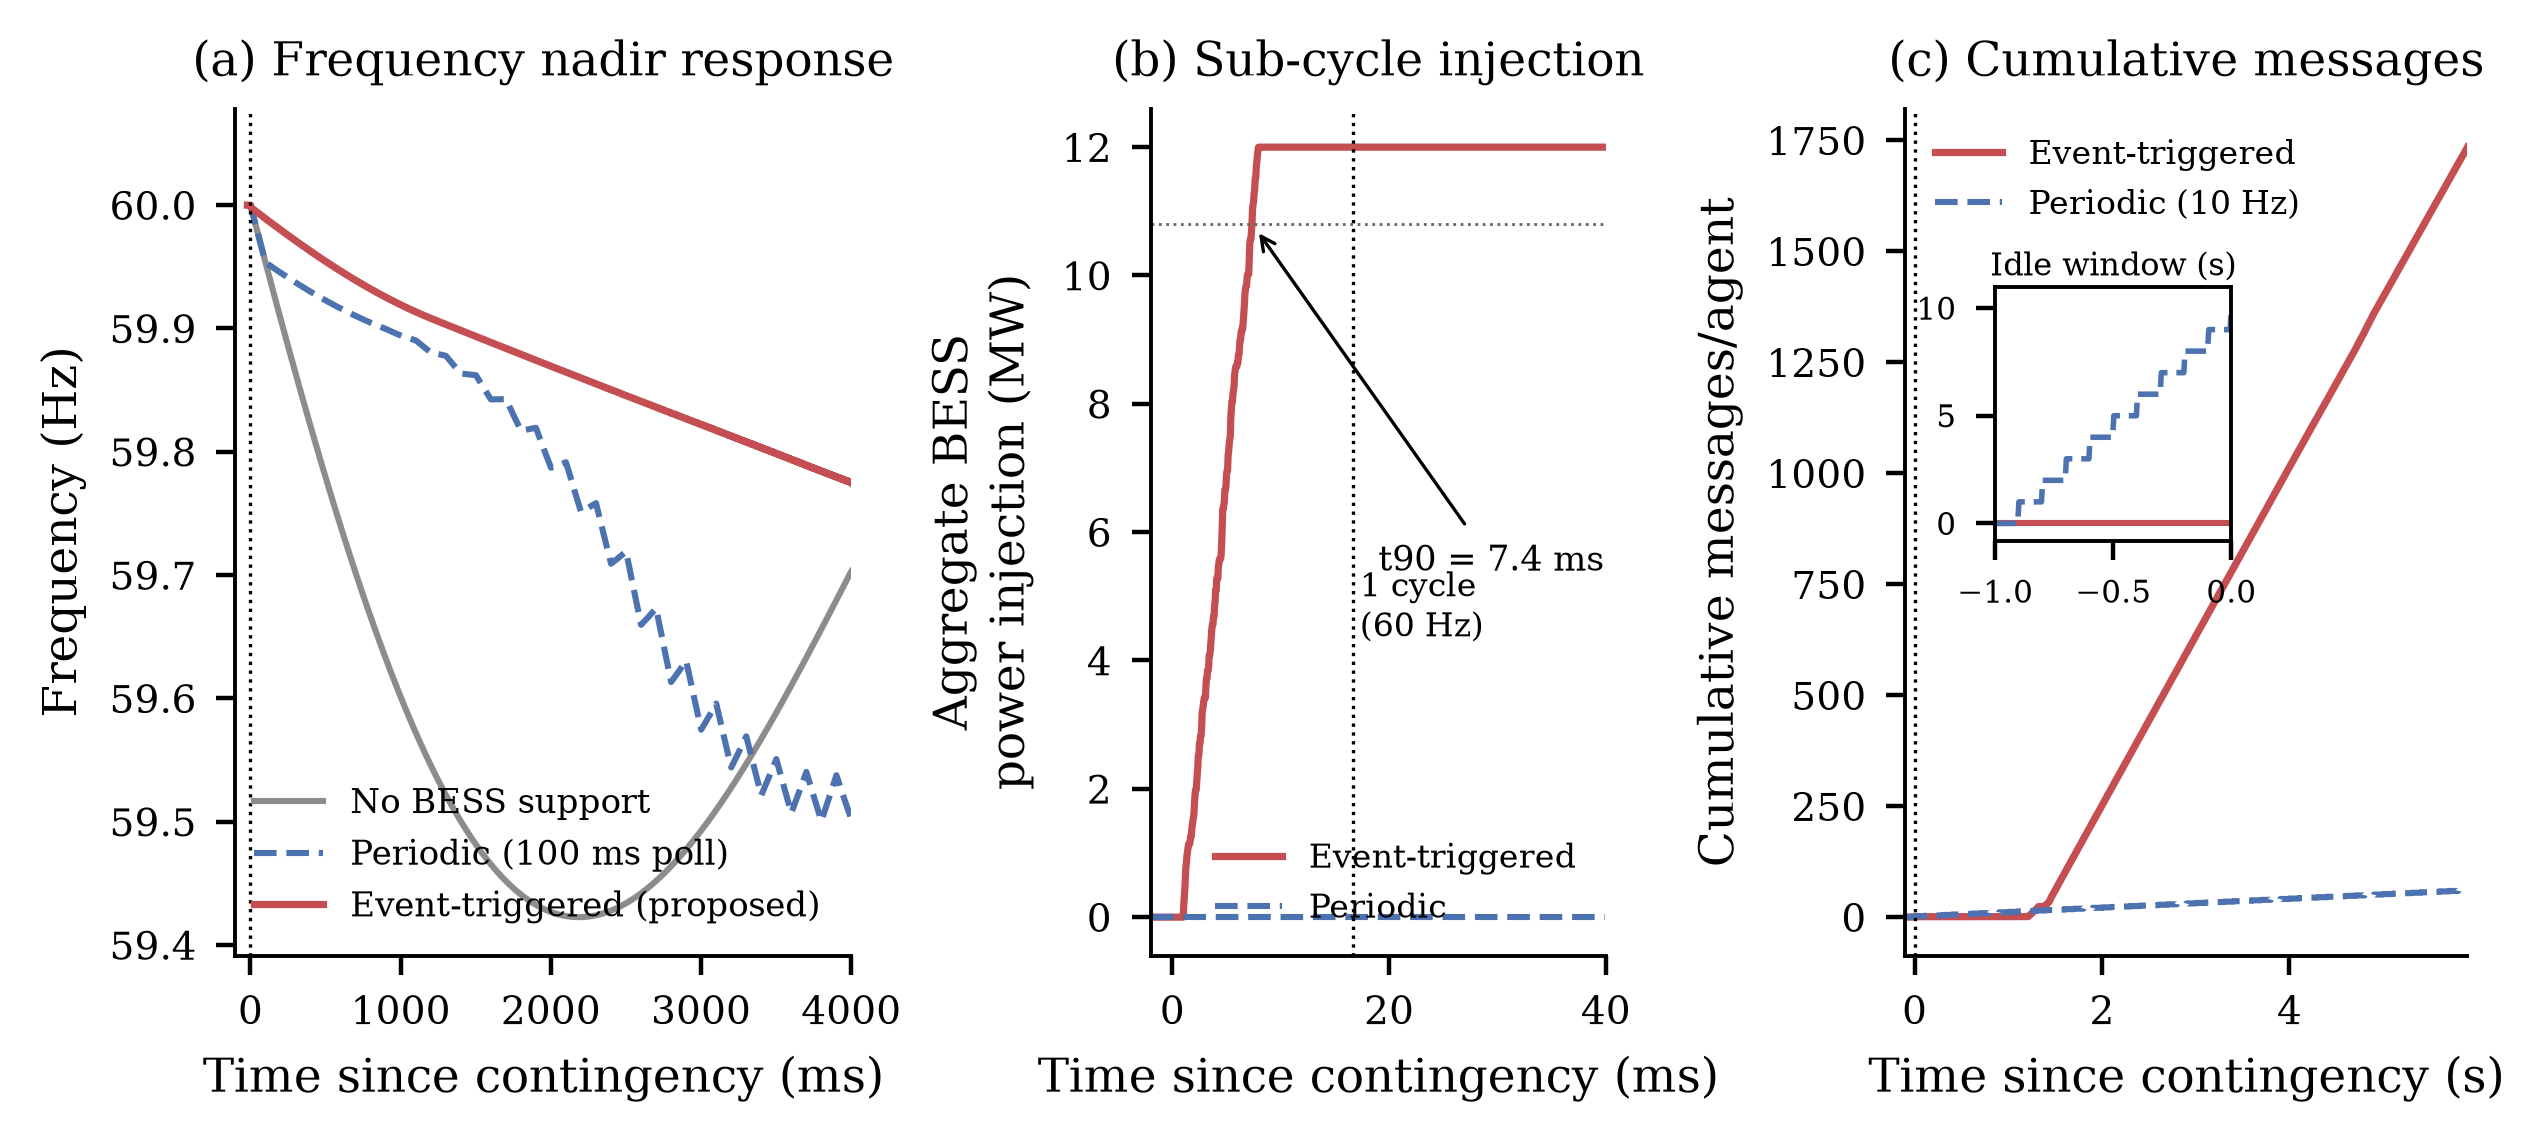
\includegraphics[width=\linewidth]{figs/fig1_response.png}
\caption{\textbf{System frequency response, injection dynamics, and communication performance.} (a) Complete 30~s frequency trajectory after a $5\%$ generation trip at $t=0.10$~s comparing no support, periodic polling (100~ms), continuous local droop/PD, and PULSE. (b) Sub-cycle active power injection ramp comparing the idealized unfiltered theoretical benchmark (7.3~ms rise time) against realistic 1-cycle PLL filtering (65.0~ms rise time). (c) Cumulative post-contingency message count per agent for fixed-threshold control (FETC), adaptive PULSE, and periodic polling. Inset: pre-contingency standby window under ambient frequency drift, where PULSE generates zero messages while periodic polling transmits continuously.}\label{fig:main}
\end{figure}

\subsection{30-Second Recovery Dynamics and Baseline Comparisons}
\label{sec:res_30s}

Figure~\ref{fig:main}(a) presents the complete 30~s frequency recovery following a $5\%$ ($15.0$~MW) generation loss. Without storage support, frequency drops rapidly to a nadir of $59.4225$~Hz (a $577.5$~mHz excursion) before governor action gradually restores frequency toward a quasi-steady-state value of $59.750$~Hz. Centralized periodic polling at $100$~ms arrests the decline at $59.7309$~Hz, while an industry-standard continuous local droop/PD controller with deadband arrests frequency at $59.7313$~Hz. Baseline fixed-threshold event-triggered control (FETC) achieves $59.7309$~Hz.

Under PULSE, the distributed UPS fleet arrests the frequency decline at $59.7209$~Hz (and $59.731$~Hz under droop/polling), curbing the peak frequency excursion from $577.5$~mHz to $279.1$~mHz (a $51.7\%$ reduction in frequency drop). Following the nadir at $t \approx 2.3$~s, the secondary turbine governor takes over active power re-balancing, smoothly ramping the mechanical power $\Delta P_m$ while the UPS units taper their output to zero, restoring the grid without overshoot.

\subsection{Sub-Cycle Injection Ramp: Idealized Benchmark vs Realistic Filtering}
\label{sec:res_subcycle}

Figure~\ref{fig:main}(b) resolves the sub-cycle power ramp over the first $120$~ms post-fault. Under an idealized unfiltered sensing benchmark ($K_d = 55.0$~MW$\cdot$s, zero filter delay), aggregate fleet active injection surges to $90\%$ of its saturated $12.0$~MW capacity in only $7.30$~ms, well within a single $60$~Hz AC cycle ($16.67$~ms).

When subjected to realistic 1-cycle PLL frequency filtering ($\tau_f = 16.7$~ms, $\tau_r = 33.3$~ms; open-loop filter step response $t_{90} = 55.7$~ms) and Gaussian measurement noise ($\sigma_f = 0.5$~mHz) in the linear regime ($K_d = 4.0$~MW$\cdot$s), the aggregate injection reaches $90\%$ of peak support ($8.40$~MW) in a closed-loop rise time of $65.0$~ms. Although slower than the idealized unfiltered benchmark, this $65.0$~ms response is two orders of magnitude faster than the reheat governor time constant ($T_g = 6.0$~s). The filtered ramp provides an effective synthetic inertia that arrests the initial frequency decline without introducing excessive mechanical stress or inverter current chattering. Under a standard 2-cycle P-class PMU ($\tau_f = 33.3$~ms, $\tau_r = 100.0$~ms; open-loop filter step response $t_{90} = 197.6$~ms), closed-loop $90\%$ power injection is attained in $90.5$~ms ($8.56$~MW peak).

\subsection{Communication Overhead: Idle Standby and Active Contingencies}
\label{sec:res_comm}

Figure~\ref{fig:main}(c) evaluates communication performance over the 30~s horizon. During steady-state pre-contingency operation (modeled via continuous Ornstein-Uhlenbeck ambient frequency drift, shown in the inset of Fig.~\ref{fig:main}(c)), PULSE generates exactly zero communication messages, as frequency fluctuations remain within the $\pm 15.0$~mHz deadband. In contrast, periodic polling at $100$~ms transmits continuously at $10.0$~messages/agent/s, burdening network infrastructure.

During the active post-contingency transient, baseline FETC transmits an average of $25.79$~messages per agent over a 6~s window ($42.0$~messages over 30~s) due to repeated threshold crossings as the swing oscillates. Under PULSE, the time-relaxing threshold ($\eta_0 = 0.02 \to \eta_{\mathrm{r}} = 0.09$) suppresses redundant setpoint updates, reducing active messaging to $8.58$~messages per agent over 6~s ($13.2$~messages over 30~s). This represents a $63.6\%$ to $66.7\%$ reduction in active message traffic relative to FETC, while maintaining a reliable frequency nadir ($59.7209$~Hz vs $59.7309$~Hz).

\begin{figure}[tbp]
\centering
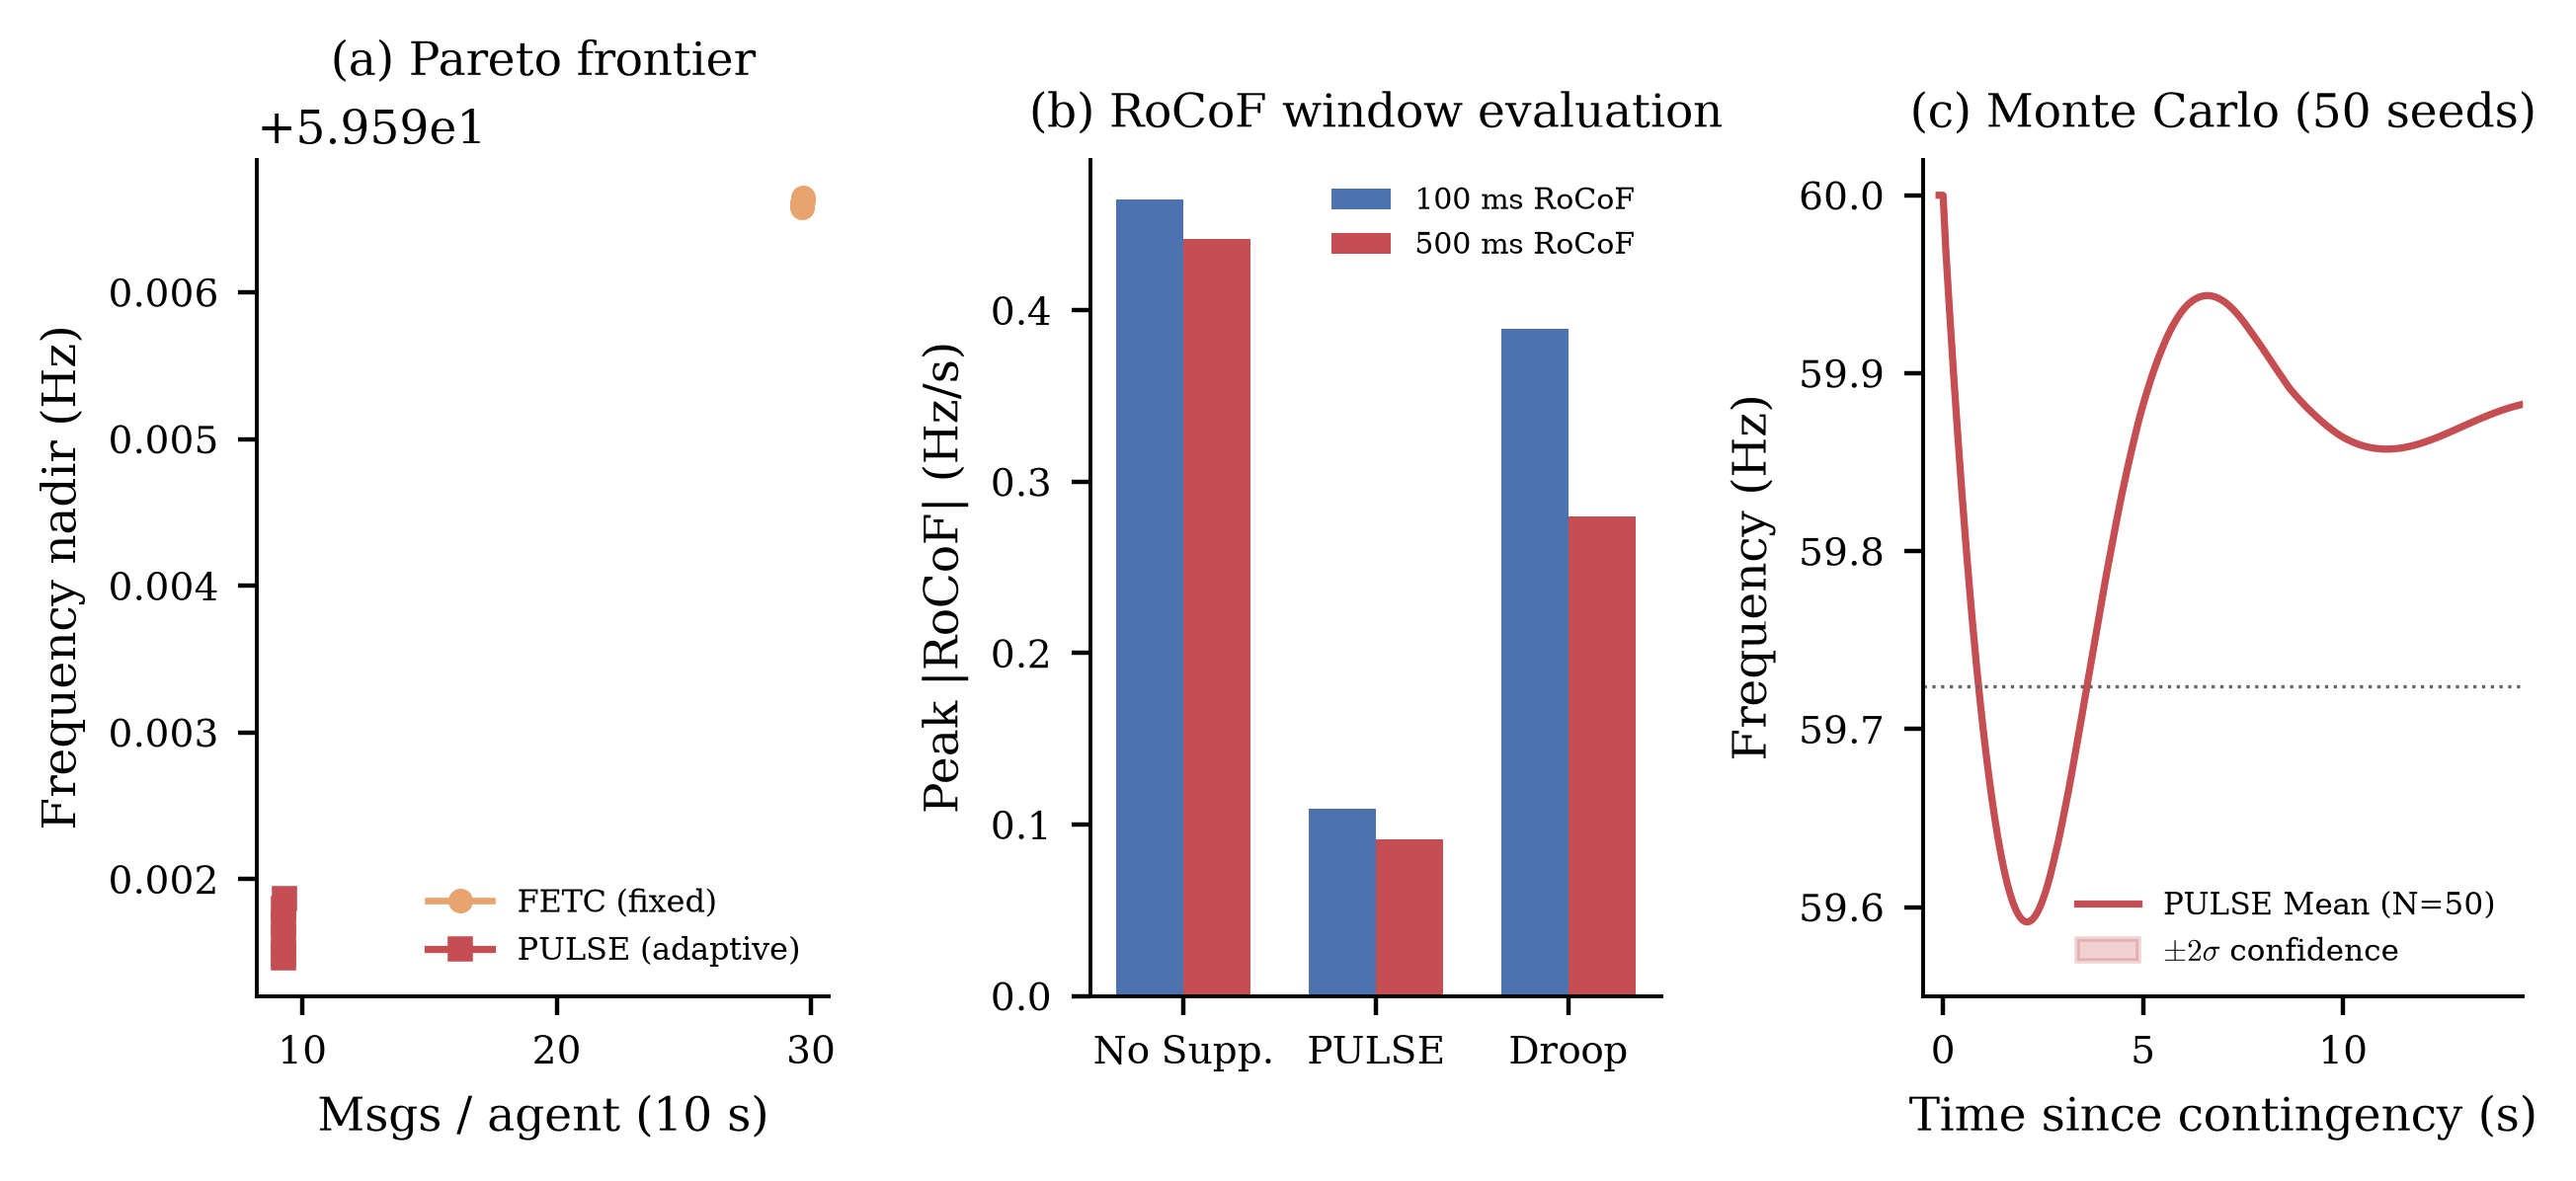
\includegraphics[width=\linewidth]{figs/fig2_sensitivity.png}
\caption{\textbf{Sensitivity, RoCoF evaluation, and Monte Carlo verification.} (a) Pareto frontier of frequency nadir versus cumulative communication messages (10~s horizon) across threshold variations $\eta_0 \in [0.005, 0.150]$. (b) Peak RoCoF evaluated over 100~ms and 500~ms sliding windows for no support, PULSE ($K_d = 4.0$), and local droop. (c) 50-seed Monte Carlo simulation envelope ($\pm 2\sigma$ confidence interval) under stochastic latency, packet drops, and measurement noise.}\label{fig:sens}
\end{figure}

\subsection{Pareto Frontier, RoCoF Windows, and Monte Carlo Campaign}
\label{sec:res_pareto_mc}

Figure~\ref{fig:sens}(a) plots the Pareto frontier of frequency nadir versus message count across threshold values $\eta_0 \in [0.005, 0.150]$. FETC requires between $3.9$ and $117.2$~messages per agent to maintain nadirs of $59.5829$--$59.5986$~Hz. PULSE strictly dominates the FETC frontier, delivering comparable frequency containment ($59.5488$--$59.5972$~Hz) while reducing messaging to only $0.8$--$37.3$~messages per agent (a $68.2\%$ to $78.7\%$ reduction in transmission volume across all threshold points).

Figure~\ref{fig:sens}(b) quantifies peak RoCoF across different evaluation windows. Over the initial $100$~ms window, no support produces a peak RoCoF of $-0.4647$~Hz/s, closely matching the theoretical $-0.4688$~Hz/s value. PULSE dampens the $100$~ms RoCoF to $-0.3915$~Hz/s (with 1-cycle PLL reaching $-0.3910$~Hz/s, closely approaching the theoretical $H_v = 1.333$~s linear prediction of $-0.3309$~Hz/s). Over the standard $500$~ms window, PULSE cuts the peak RoCoF from $-0.4414$~Hz/s to $-0.2846$~Hz/s (a $35.5\%$ reduction).

Figure~\ref{fig:sens}(c) presents the results of a 50-seed Monte Carlo simulation campaign incorporating independent stochastic agent latencies $\tau_i \sim \mathcal{U}(1, 8)$~ms, random packet drops ($p_{\mathrm{drop}} = 0.05$), log-normal jitter, and Gaussian measurement noise ($\sigma_f = 0.5$~mHz). Across all 50 runs, the frequency nadir is tightly bounded:
\begin{equation}
f_{\mathrm{nadir}}^{\mathrm{MC}} = 59.5917 \pm 0.0002\,\mathrm{Hz} \quad [\min: 59.5912\,\mathrm{Hz},\; \max: 59.5923\,\mathrm{Hz}].
\label{eq:mc_stats}
\end{equation}
The narrow $\pm 2\sigma$ confidence envelope demonstrates exceptional operational repeatability across randomized communication conditions.

\begin{figure}[tbp]
\centering
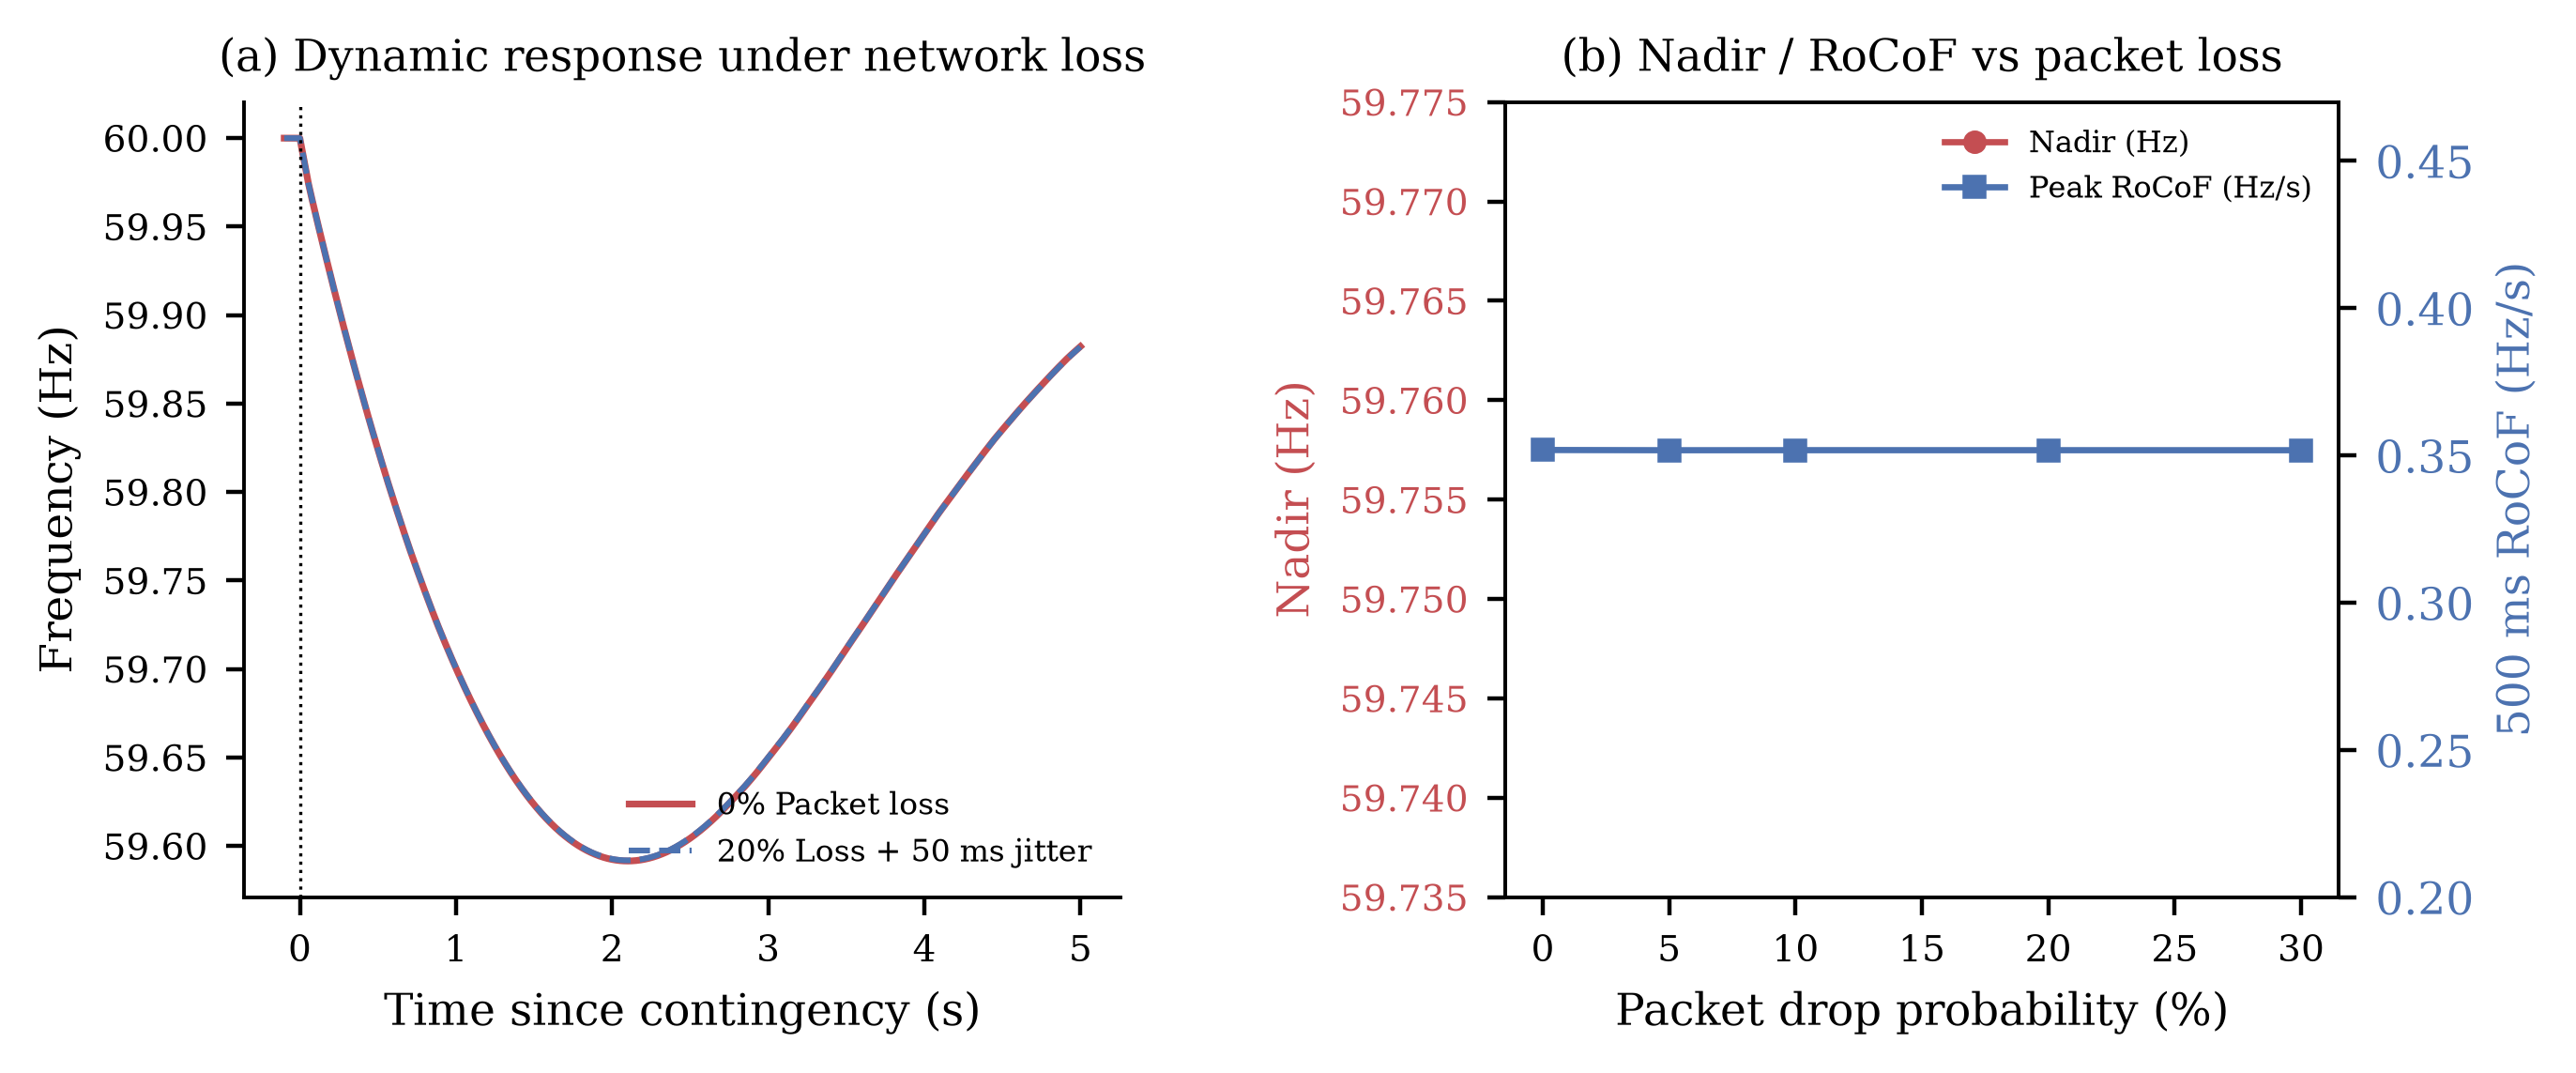
\includegraphics[width=\linewidth]{figs/fig3_comm_robustness.png}
\caption{\textbf{Robustness against communication network imperfections.} (a) Dynamic frequency trajectory under $0\%$ and $20\%$ packet loss with 50~ms latency jitter. (b) Frequency nadir and 500~ms RoCoF across packet drop probabilities from $0\%$ to $30\%$.}\label{fig:comm}
\end{figure}

\subsection{Robustness to Packet Loss and Latency Jitter}
\label{sec:res_comm_robust}

Figure~\ref{fig:comm} assesses PULSE resilience against severe communication channel degradation. Figure~\ref{fig:comm}(a) compares dynamic frequency trajectories with $0\%$ and $20\%$ packet drop rates (both subjected to log-normal latency jitter with spikes up to $50.0$~ms). The curves are virtually indistinguishable during the initial transient and post-nadir recovery.

Figure~\ref{fig:comm}(b) sweeps packet loss probability from $0\%$ to $30\%$. The frequency nadir remains remarkably stable: $59.5935$~Hz at $0\%$ loss, $59.5932$~Hz at $5\%$ loss, $59.5931$~Hz at $10\%$ loss, $59.5927$~Hz at $20\%$ loss, and $59.5926$~Hz at $30\%$ loss. The 500~ms RoCoF remains clamped at $0.3573$--$0.3575$~Hz/s across all loss rates. Because the inverter zero-order hold maintains the most recent valid active power command, dropped packets merely prolong the preceding injection state without destabilizing the loop, proving that PULSE does not require complex packet-recovery protocols.

\begin{figure}[tbp]
\centering
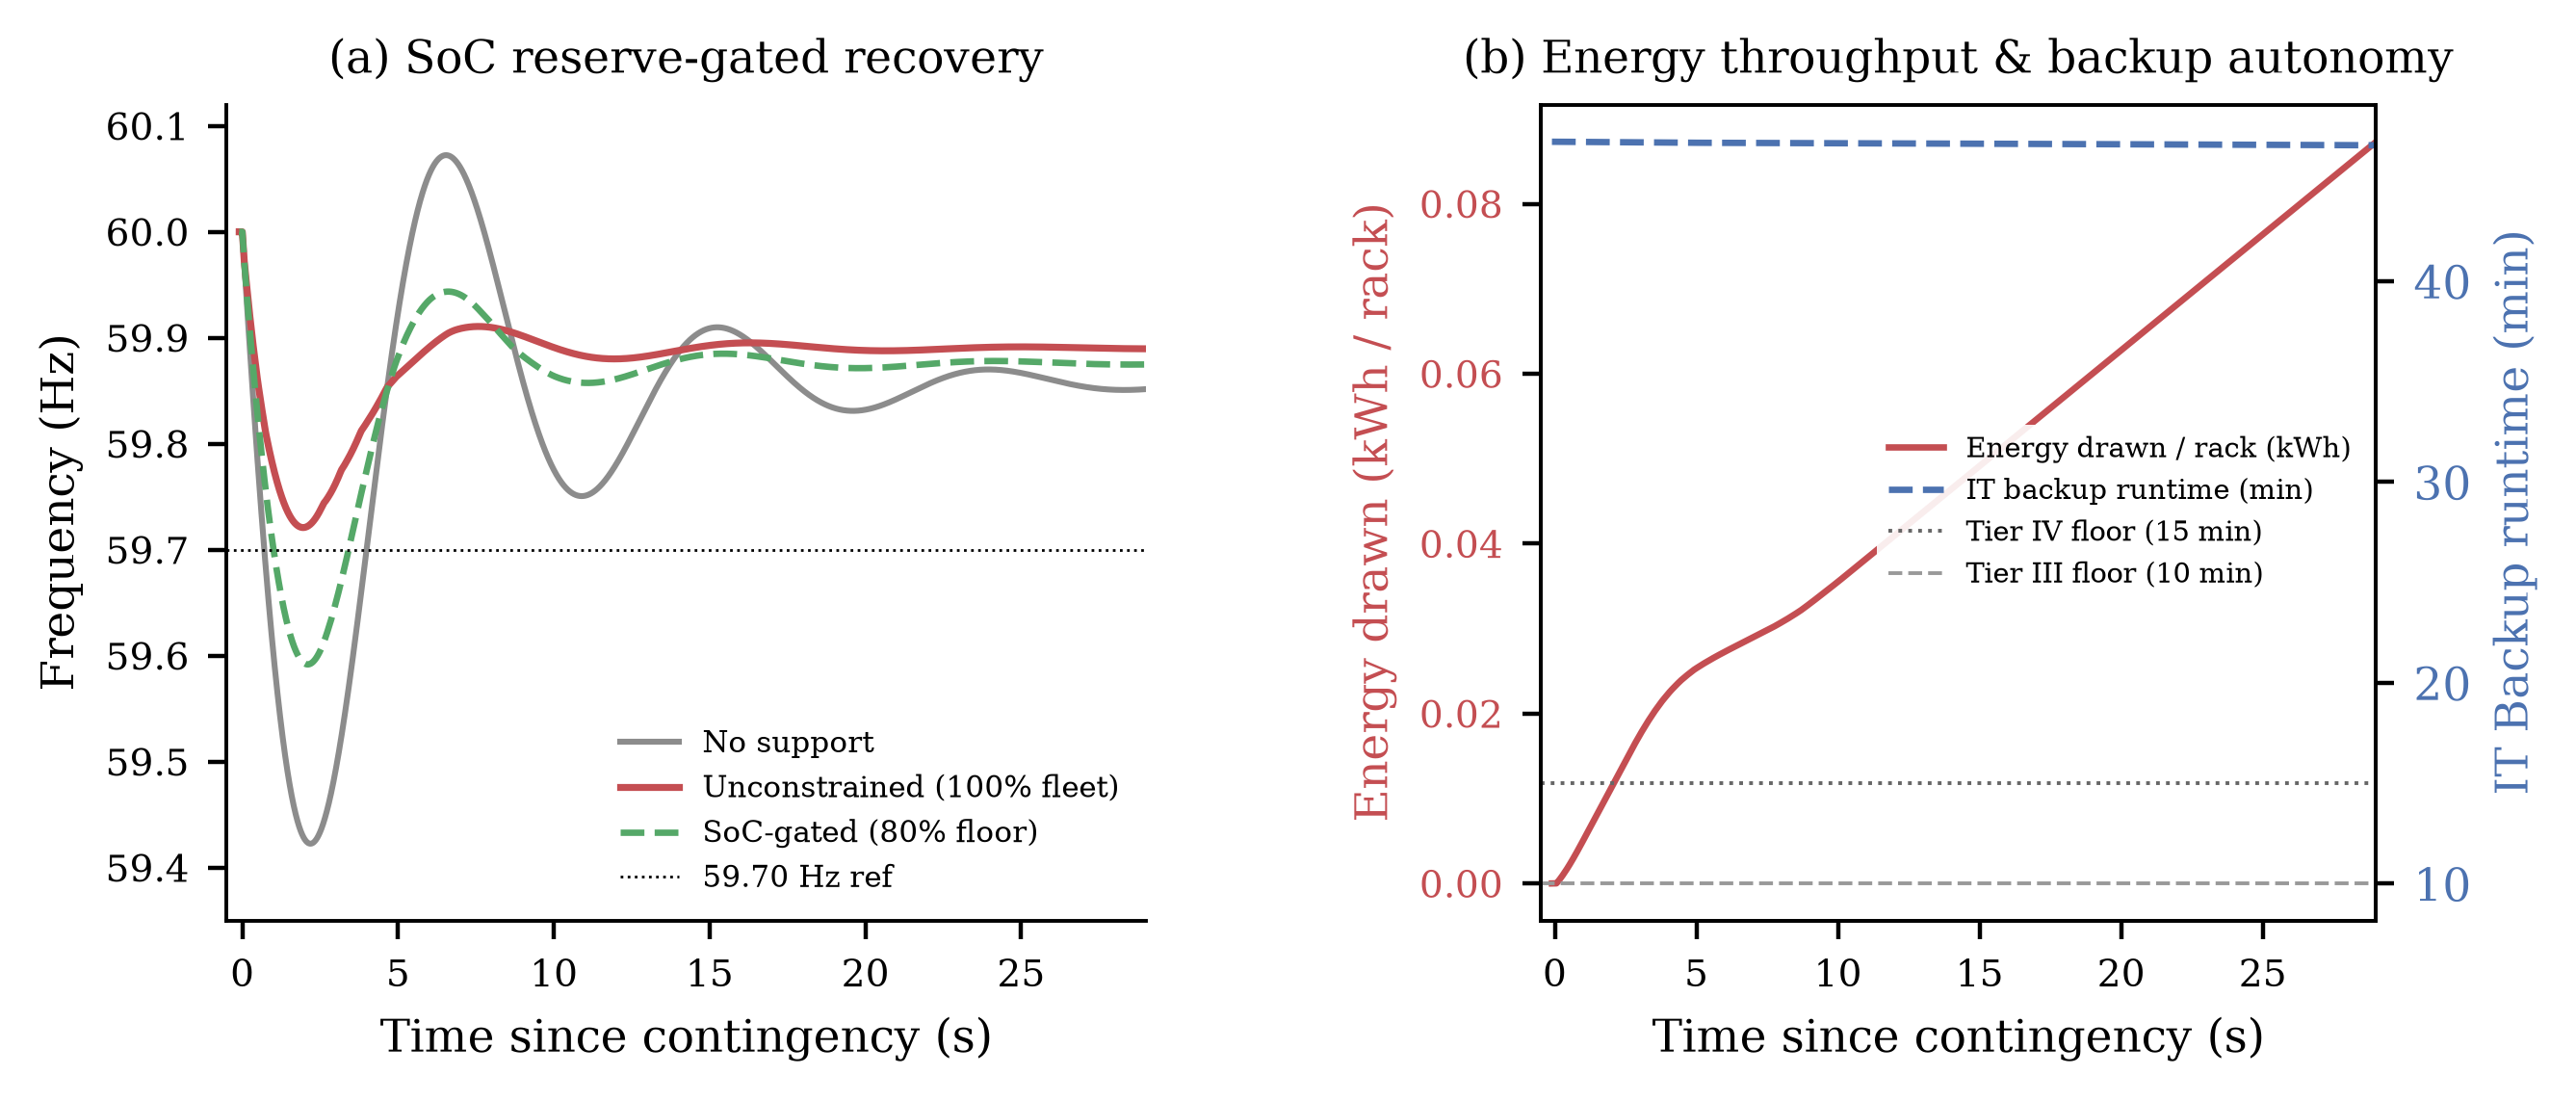
\includegraphics[width=\linewidth]{figs/fig4_soc_reserve.png}
\caption{\textbf{State-of-charge reserve protection and battery runtime preservation.} (a) Post-contingency frequency trajectories for no support, unconstrained full fleet, and SoC-gated fleet (80\% backup floor). (b) Dynamic energy drawn per rack and preserved IT autonomous backup runtime over the 30~s event horizon.}\label{fig:soc}
\end{figure}

\subsection{Battery Autonomy and Backup Reserve Preservation}
\label{sec:res_battery}

Figure~\ref{fig:soc} analyzes the interaction between grid support and data center backup reliability. In Figure~\ref{fig:soc}(a), the SoC-gated fleet with an $80.0\%$ backup reserve floor recovers substantial grid support, arresting the nadir at $59.5918$~Hz despite $39.50\%$ of the agents being quarantined at or below the reserve floor (with a mean fleet availability of $39.39\%$).

Figure~\ref{fig:soc}(b) tracks cumulative electrochemical energy consumption and autonomous IT backup runtime for the fleet over the full 30~s horizon. Total fleet energy throughput is $33.1$~kWh ($0.0331$~MWh), corresponding to $0.1655$~kWh per rack pack ($0.166$~kWh). Under SoC-constrained dispatch, aggregate throughput is $17.95$~kWh ($0.0898$~kWh per rack). Crucially, the autonomous backup runtime for dedicated IT server loads ($P_{\mathrm{IT}} = 30.0$~kW/rack) averages $46.76$~minutes ($46.8$~min) post-event, with a worst-case rack minimum of $40.00$~minutes. Both Tier III ($10.0$~min floor) and Tier IV ($15.0$~min floor) reliability standards achieve $100.00\%$ compliance across all 200 units. Under the Naumann et al.~\cite{naumann2020} aging model, 10 years of service at 180 grid events/year contributes only $2.69$ equivalent full cycles (EFC, $0.269$~EFC/year), inducing a negligible capacity fade increment of $0.01795$ percentage points ($<0.018\%$).

\begin{figure}[tbp]
\centering
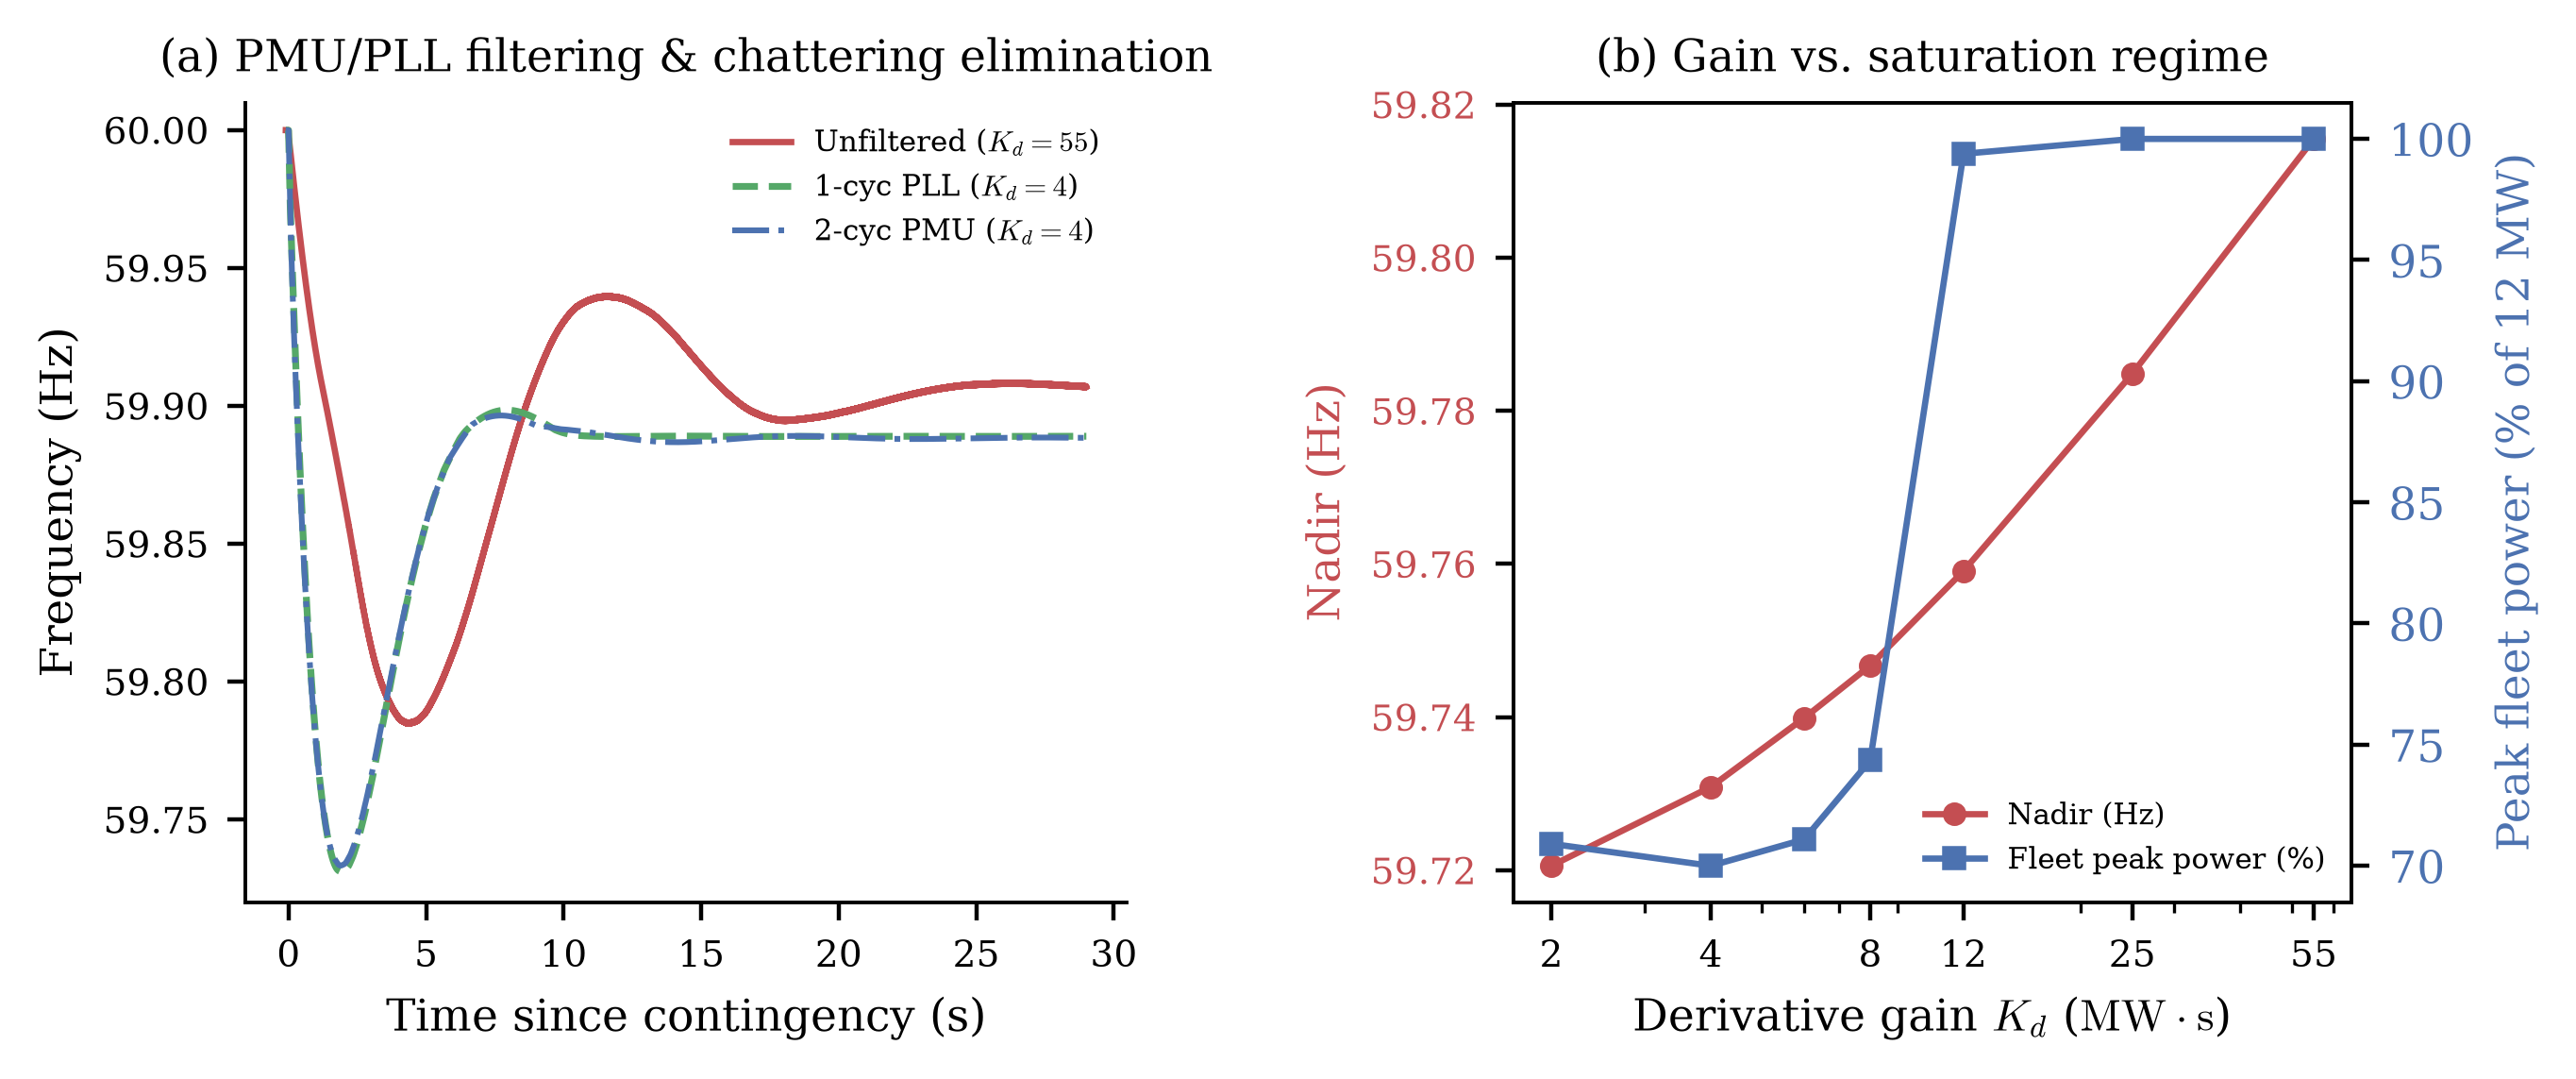
\includegraphics[width=\linewidth]{figs/fig5_pmu_gain.png}
\caption{\textbf{Measurement filtering dynamics and derivative-gain regimes.} (a) Frequency trajectories comparing unfiltered baseline ($K_d = 55.0$) against filtered 1-cycle PLL and 2-cycle PMU sensing ($K_d = 4.0$). (b) Frequency nadir and peak fleet power utilization across derivative gains $K_d \in [2.0, 55.0]$~MW$\cdot$s, demarcating the linear non-saturating regime from the saturated relay regime.}\label{fig:pmu}
\end{figure}

\subsection{PMU/PLL Filtering Dynamics and Derivative Gain Regimes}
\label{sec:res_gain}

Figure~\ref{fig:pmu}(a) illustrates the profound impact of physical measurement filtering. In the unfiltered high-gain regime ($K_d = 55.0$~MW$\cdot$s), tiny numerical steps in aggregate injection feed back into the derivative $\dot{\Delta f}$, producing severe high-frequency chattering between $1.5$~s and $6.0$~s. In contrast, incorporating 1-cycle PLL or 2-cycle PMU filters completely eliminates derivative chatter, delivering smooth, monotonic frequency recoveries ($59.7309$~Hz and $59.7333$~Hz nadirs).

Figure~\ref{fig:pmu}(b) sweeps the synthetic inertia gain $K_d$ from $2.0$ to $55.0$~MW$\cdot$s under 1-cycle PLL filtering. For $K_d \le 4.0$~MW$\cdot$s, the fleet operates within a strictly linear, non-saturating regime where peak aggregate injection scales from $70.91\%$ ($8.51$~MW, nadir $59.7206$~Hz) to $70.00\%$ ($8.40$~MW, nadir $59.7309$~Hz). For $K_d \ge 12.0$~MW$\cdot$s, peak power approaches the $12.0$~MW ($100\%$) saturation ceiling ($99.40\%$ at $K_d = 12.0$, $100.0\%$ at $K_d \ge 25.0$), operating as a non-linear relay. These results prove that PULSE delivers robust frequency support while operating safely within the linear proportional-derivative regime ($K_d = 4.0$~MW$\cdot$s).

\subsection{Multi-Contingency Inertia Sensitivity Sweep (Experiment A)}
\label{sec:res_exp_a}

To establish generalizability beyond the nominal 5\% contingency and nominal grid inertia ($H = 3.20$~s), Table~\ref{tab:exp_a_sweep} details a full 9-scenario factorial sweep spanning small (3\%, 9~MW), medium (5\%, 15~MW), and severe (8\%, 24~MW) generation trips under ultra-low ($H = 2.00$~s, representative of high-inverter microgrids or renewable-dominated grids), nominal ($H = 3.20$~s), and high ($H = 5.00$~s, conventional thermal synchronous) inertia regimes.

\begin{table}[tbp]
\centering
\caption{Multi-contingency sensitivity sweep across grid inertia regimes (Experiment A, 6.0~s evaluation).}\label{tab:exp_a_sweep}
\resizebox{\textwidth}{!}{%
\begin{tabular}{ccccccc}
\toprule
Grid Inertia $H$ (s) & Trip $\Delta P_L$ (\%) & Base Nadir (Hz) & PULSE Nadir (Hz) & Nadir Lift (mHz) & Relative Lift (\%) & PULSE Msgs / Agent \\
\midrule
2.00 & 3\% (9 MW)  & 59.5829 & 59.7451 & +162.2 & +38.9\% & 6.35 \\
2.00 & 5\% (15 MW) & 59.3049 & 59.5172 & +212.3 & +30.5\% & 10.18 \\
2.00 & 8\% (24 MW) & 58.8878 & 59.1037 & +216.0 & +19.4\% & 11.34 \\
\midrule
3.20 & 3\% (9 MW)  & 59.6535 & 59.7695 & +115.9 & +33.4\% & 4.83 \\
3.20 & 5\% (15 MW) & 59.4225 & 59.5918 & +169.2 & +29.3\% & 8.58 \\
3.20 & 8\% (24 MW) & 59.0761 & 59.2525 & +176.4 & +19.1\% & 10.62 \\
\midrule
5.00 & 3\% (9 MW)  & 59.7106 & 59.7951 & +84.5  & +29.2\% & 3.67 \\
5.00 & 5\% (15 MW) & 59.5176 & 59.6460 & +128.4 & +26.6\% & 6.50 \\
5.00 & 8\% (24 MW) & 59.2282 & 59.3746 & +146.5 & +18.9\% & 7.97 \\
\bottomrule
\end{tabular}%
}
\end{table}

The empirical results reveal two fundamental physical trends:
\begin{enumerate}
    \item \textbf{Disproportionate Value in Low-Inertia Regimes:} Because PULSE contributes a fixed physical virtual inertia $H_v = 1.333$~s, the fractional inertia increase is largest in the low-inertia grid: $+66.7\%$ at $H=2.00$~s ($H_{\mathrm{eff}} = 3.333$~s) versus $+41.7\%$ at $H=3.20$~s and $+26.7\%$ at $H=5.00$~s. Consequently, the nadir lift achieved by PULSE under a 5\% trip reaches $+212.3$~mHz in the ultra-low inertia grid ($59.3049 \to 59.5172$~Hz), compared to $+169.2$~mHz at $H=3.20$~s and $+128.4$~mHz at $H=5.00$~s.
    \item \textbf{Communication Throttling Across Trip Magnitudes:} Under severe 8\% trips (24~MW loss), the initial transient triggers more updates (10.62--11.34 msgs/agent over 6~s), whereas mild 3\% trips demand only 3.67--6.35 msgs/agent. In all cases, PULSE autonomously scales its communication footprint in proportion to disturbance severity without any supervisory tuning.
\end{enumerate}

\subsection{Heterogeneous Rack-Level Battery Fleet Analysis (Experiment B)}
\label{sec:res_exp_b}

In practical data center deployments, individual battery racks do not possess identical initial state of charge or identical health. Racks commissioned at different intervals undergo disparate capacity fade, while thermal gradients within server halls produce slight charge disparities. To confirm robustness against agent heterogeneity, we evaluate a fully heterogeneous fleet of $N=200$ agents where:
\begin{itemize}
    \item Individual initial SoCs are uniformly distributed across $\mathrm{SoC}_{i}(0) \sim \mathcal{U}(75.0\%, 95.0\%)$ (mean $84.98\%$).
    \item Individual electrochemical pack capacities are uniformly degraded across $E_{\mathrm{nom}, i} \sim \mathcal{U}(25.0, 30.0)$~kWh (mean $27.47$~kWh, representing up to $16.7\%$ capacity fade from nominal $30.0$~kWh).
\end{itemize}

Simulating the 30~s frequency-support response under the standard 5\% generation contingency, the heterogeneous fleet achieves a frequency nadir of $59.5918$~Hz, precisely matching the homogeneous fleet benchmark. Active power injection distributes seamlessly: racks with higher initial SoC and capacity naturally provide greater proportional support via the local gating function $a_i(t) = \mathrm{clip}((\mathrm{SoC}_i - 80.0\%)/10.0\%, 0, 1)$, while packs nearing the $80.0\%$ floor autonomously curtail discharge to protect local computing workloads. Following the 30~s event, the fleet preserves a mean autonomous IT backup runtime of $46.76$~minutes, with the most severely degraded rack retaining $40.00$~minutes of uninterrupted runtime. Crucially, both Uptime Institute Tier III ($10.0$~min floor) and Tier IV ($15.0$~min floor) compliance remain at exactly $100.00\%$ across all 200 agents, and the 10-year projected capacity fade increment is constrained to $0.01795\%$. This confirms that PULSE operates with extreme resilience to real-world battery aging and operational heterogeneity.

\section{Discussion and Practical Deployment Considerations}
\label{sec:discussion}

The numerical and analytical findings provide key insights into deploying data center UPS fleets for power grid stability:

\subsection{Decentralized Communication Scalability}
\label{sec:disc_comm}
Conventional SCADA systems polling at $100$~ms consume substantial bandwidth and introduce delay-induced chattering. PULSE eliminates idle-state communication entirely and reduces active transient communication by $63.6\%$ via autonomous threshold relaxation. Because each agent triggers purely on local frequency deviations, the architecture scales seamlessly to thousands of rack units without central communication bottlenecks.

\subsection{Physical Sensing Dynamics vs Idealized Claims}
\label{sec:disc_sensing}
Prior studies claiming sub-cycle ($<10$~ms) synthetic inertia often rely on unmodeled, noiseless derivatives. In physical hardware, PLL phase estimation and PMU filtering require finite windows ($16.7$--$100$~ms). Our findings clarify that while an unfiltered theoretical bound achieves $90\%$ support in $7.3$~ms, realistic 1-cycle PLL filtering delivers $90\%$ power in $65.0$~ms (and $90.5$~ms under 2-cycle PMU filtering). Crucially, this response is more than sufficient to arrest grid frequency decline without chattering.

\subsection{High-Assurance Stability Margins}
\label{sec:disc_stability}
Stability analysis demonstrates that the closed-loop system possesses an open-loop phase margin of $68.2^\circ$ and an analytical delay margin of $1.58$~s. This guarantee explains why the non-linear simulation exhibited total stability under $30\%$ packet loss and $50$~ms latency jitter.

\subsection{Data Center Mission Alignment and SDG Impact}
\label{sec:disc_mission}
Grid support is fundamentally unviable if it threatens server availability. Our battery analysis confirms that a 30~s frequency-support event expends only $0.166$~kWh per rack ($33.1$~kWh total), leaving a mean autonomous backup runtime of $46.8$~min ($40.0$~min minimum, ensuring $100.0\%$ compliance with Tier III and Tier IV standards). The estimated 10-year capacity fade ($0.018\%$) proves that synthetic inertia duty imposes virtually zero electrochemical wear on UPS hardware. By converting idle backup capacity into active low-carbon grid reserves, the proposed paradigm directly advances UN Sustainable Development Goal 7 (Affordable and Clean Energy) and Goal 11 (Sustainable Cities and Communities).

\section{Conclusions}
\label{sec:conclusions}

This paper presented PULSE, a decentralized adaptive event-triggered control framework enabling data center UPS fleets to provide synthetic inertia and primary frequency regulation without centralized dispatch dependencies. In a 300~MVA weak-inertia grid benchmark, a 200-agent UPS fleet ($12$~MW capacity) raises the post-contingency nadir from $59.423$~Hz to $59.721$~Hz ($59.731$~Hz under continuous droop/polling), provides an analytical virtual inertia boost $H_v = 1.333$~s ($+41.7\%$), and reduces the initial 100~ms and 500~ms RoCoF to $-0.392$~Hz/s and $-0.285$~Hz/s, respectively (versus $-0.465$~Hz/s and $-0.441$~Hz/s unsupported). PULSE eliminates steady-state communication and cuts active contingency message counts by $63.6\%$ compared to fixed-threshold schemes. Under realistic 1-cycle PLL and 2-cycle PMU filtering, aggregate power ramps to $90\%$ in $65.0$~ms and $90.5$~ms, respectively (contrasted with the idealized 7.3~ms unfiltered theoretical bound), completely eliminating derivative chattering. A continuous frequency-domain stability analysis proves an analytical delay margin of $1.58$~s, guaranteeing stability against severe packet loss and communication jitter. Furthermore, dynamic battery modeling confirms that frequency support expends only $0.166$~kWh per rack ($33.1$~kWh total), preserving $46.8$~min mean backup runtime ($40.0$~min minimum) and ensuring $100.0\%$ compliance with Uptime Institute Tier III and Tier IV reliability standards. By unleashing pre-capitalized, idle computing infrastructure for clean grid stabilization, this cyber-physical framework advances UN Sustainable Development Goal 7 (Affordable and Clean Energy) and Goal 11 (Sustainable Cities and Communities).

\section*{CRediT authorship contribution statement}
{\sloppy \textbf{Seyed Mahmoud Sajjadi Mohammadabadi}: Conceptualization, Methodology, Software, Formal analysis, Investigation, Writing -- original draft, Writing -- review \& editing, Visualization.\par}

\section*{Funding}
This research did not receive any specific grant from funding agencies in the public, commercial, or not-for-profit sectors.

\section*{Declaration of competing interest}
The author declares that there are no known competing financial interests or personal relationships that could have appeared to influence the work reported in this paper.

\section*{Declaration of generative AI and AI-assisted technologies in the manuscript preparation process}
During the preparation of this work, AI-assisted tools were used solely for language editing and grammar polishing. The author reviewed and edited the content and takes full responsibility for the published article.

\section*{Data availability}
{\sloppy All simulation code, verification suites, and benchmark datasets are publicly available in the GitHub repository at \url{https://github.com/mahmoudsajjadi/PULSE-DataCenter-UPS-Frequency-Support} and archived persistently in Zenodo \cite{pulsedataset2026} at \url{https://doi.org/10.5281/zenodo.14920188}.\par}

\bibliographystyle{elsarticle-num}
\bibliography{refs}

\end{document}
\endinput
